\documentclass[a4paper,12pt]{article}
\usepackage[utf8]{inputenc} % Codificação para caracteres especiais
\usepackage{graphicx}       % Para incluir imagens
\usepackage{geometry}       % Para ajustar margens
\usepackage[linesnumbered, ruled, vlined]{algorithm2e}
\usepackage{caption}
\usepackage{indentfirst} %pacote que faz indentação na primeira linha do parágrafo
\usepackage{hyperref}
\usepackage{breakurl}
\usepackage{xurl}
\usepackage{float}
\usepackage{amsmath}
\usepackage{subcaption}
\usepackage{array}
\newcolumntype{C}[1]{>{\centering\arraybackslash}p{#1}}

\hypersetup{breaklinks=true}
\setlength{\parindent}{1cm} %pacote que define o tamanho da indentação
\captionsetup[figure]{labelfont=bf}
\usepackage[portuguese]{babel}
\usepackage{longtable}
\usepackage{booktabs}




%Permite quebras de página para blocos de matemática
\allowdisplaybreaks[4]
% Ajustes de hifenização e espaçamento
\hyphenpenalty=10000
\exhyphenpenalty=10000
\sloppy

\hypersetup{
    colorlinks=true,       % Ativa a cor dos links
    linkcolor=black,       % Cor dos links internos (sumário, referências, etc.)
    urlcolor=blue,         % Cor dos links externos (como o URL do GitHub)
    citecolor=black        % Cor das citações (se houver)
}


% Configuração das margens
\geometry{
    top=3cm,
    bottom=2cm,
    left=3cm,
    right=2cm
}

\begin{document}
\begin{titlepage}
    \thispagestyle{empty}
    \begin{center}
        
\includegraphics[width=3cm]{images/brasao_gradiente.png} \\
        \vspace{0.5cm}
        {\large {Universidade Federal do Rio Grande do Norte}} \\
        {\large {Centro de Ciências Exatas e da Terra}} \\
        {\large {Departamento de Informática e Matemática Aplicada}} \\
        {\large {Bacharelado em Ciência da Computação}} \\
    \end{center}

    \vspace{4cm}

    \begin{center}
        {\large {Jeremias Pinheiro de Araujo Andrade}} \\
        {\large {Lucas Apolonio de Amorim}} \\
        {\large {Moisés Ferreira de Lima}} \\
    \end{center}

    \vspace{4cm}

    \begin{center}
        {\large \textbf{Resultados - POS Tagging Usando Arquiteturas Neurais}} \\
        {\large \textbf{DIM0135 - Processamento de Linguagem Natural}}
    \end{center}

    \vspace{4cm}

    \begin{center}
        {\large Natal/RN} \\
        {\large 2026}
    \end{center}
\end{titlepage}

% CONTRACAPA
\begin{titlepage}
    \thispagestyle{empty} % Remove o número da página na contracapa
    \begin{center}
        {\large {Jeremias Pinheiro de Araujo Andrade}} \\
        {\large {Lucas Apolonio de Amorim}} \\
        {\large {Moisés Ferreira de Lima}} \\
        \vspace{4cm}

        {\large {Especificação das Arquiteturas Neurais}} \\
        {\large {DIM0135 - Processamento de Linguagem Natural}}
        \vspace{6cm}
        \begin{flushright}
            \begin{minipage}{0.5\textwidth}
            Relatório discutindo os Resultados das Arquiteturas Neurais implementadas para o Projeto Final da disciplina de Processamento de Linguagem Natural, ministrada pelo professor Dr. Carlos Augusto Prolo no Curso de Ciência da Computação do Departamento de Informática e Matemática Aplicada da Universidade Federal do Rio Grande do Norte – Campus Central (Natal). \\
            \end{minipage}
        \end{flushright}
    \end{center}

    % Local e data
    \vspace{4cm}
    \begin{center}
        {\large Natal/RN} \\
        {\large 2026}
    \end{center}
\end{titlepage}


\renewcommand{\contentsname}{\begin{center}Conteúdos\end{center}}
\tableofcontents
\thispagestyle{empty}

\newpage

\setcounter{page}{3}

\section{Introdução}
O Penn Treebank é um dos Treebanks mais conhecidos e utilizados para tarefas de Processamento de Linguagem Natural, especialmente tarefas como o Part-of-Speech Tagging e Parsing da Gramática de Constituintes de uma sentença.

Nesse Relatório serão análisados os Resultados de implementações de diversas arquiteturas Neurais usadas para POS Tagging no Penn Treebank, usando a divisão padrão de treino (seções 0-18), validação (seções 19-21) e teste (seções 22-24).

\section{Desafios}

\subsection{Embeddings Pré Treinados}
Quando utilizando uma matriz de Embeddings pré treinados, precisamos garantir que eles são compatíveis com o corpus em que o nosso modelo irá operar, o que pode implicar na criação de novos tokens ou no uso de unknown words, também deve ser decidido se a camada de embedding será congelada (isso é, não será sujeitada a treinamento) ou não. Foram utilizados os Embeddings do GloVe6B sem Freeze da camada de embedding, ou seja, foram sujeitos à post-training.

\subsection{Unknown Words}
Precisamos fazer com que o modelo seja capaz de lidar com tokens que não foram vistos durante o treino ou que não estão no vocabulário do modelo (especialmente se os embeddings são palavras inteiras), para isso, criamos um token \texttt{<UNK>}, que representa essas Unknown Words, e também associamos palavras incomuns do corpus de treino com esse token para treinar o modelo a inferir uma tag de acordo com o contexto da sentença. Para os modelos baseados em Transformer e RNN, foi escolhido um tamanho fixo de vocabulário entre 10.000 palavras e 15.000 palavras, sendo a decisão de quais palavras incluir no vocabulário baseado na frequência das palavras no corpus de \textbf{treino}.

\subsection{Padding dos Inputs e Outputs}
Para lidar com sentenças de tamanho variável, devemos emular de alguma forma o comprimento de todas as sentenças para o tamanho máximo, isso costuma ser feito através da inserção de padding no final (concatenação de vários tokens \texttt{<PAD>}, que é um token especial feito para preencher espaço).

\subsection{Avaliação da Performance dos Modelos}
Não exatamente um desafio, mas sim uma decisão a ser tomada. Para avaliar os modelos de Tagging, foi medida a Acurácia para todas as tags e gerado um mapa de calor da Matriz de Confusão. São desconderados os tokens de Pad, tokens de pontuação foram contabilizados e estão inclusos na matriz de confusão

\section{Resultados}

\subsection{RNN e LSTM}

\subsubsection{Estratégia de Implementação}
A estratégia experimental para avaliar os modelos de Rede Neural Recorrente consistiu em analisar o impacto de diferentes células recorrentes e da direcionalidade no processamento de sequências para a tarefa de marcação gramatical (\textit{Part-of-Speech Tagging}). O pipeline foi estruturado nas seguintes etapas:

\begin{itemize}
    \item \textbf{Processamento dos Dados:} Os dados do \textit{Penn Treebank} foram divididos de forma determinística nos splits de Treino (38.219 sentenças), Validação (5.527 sentenças) e Teste (5.462 sentenças). O vocabulário textual foi truncado nas 8.000 palavras mais frequentes, e as sequências foram limitadas a um comprimento máximo de $max\_len = 249$ tokens.
    \item \textbf{Mapeamento de Alvos:} O espaço de busca consiste em 47 \textit{tags} únicas de POS gramaticais. O token invisível de preenchimento (\texttt{<PAD>}) foi explicitamente mapeado para o índice 0 e mascarado na camada de acoplamento do modelo para evitar a contaminação dos gradientes.
    \item \textbf{Hiperparâmetros Fixos:} Para isolar a influência das arquiteturas, todos os experimentos compartilharam um \textit{Embedding} de 128 dimensões, 128 unidades ocultas na camada recorrente, otimizador Adam, função de perda \textit{Sparse Categorical Crossentropy}, \textit{batch size} de 32 e teto estipulado de 5 épocas de treinamento.
\end{itemize}

\subsubsection{Resultados Gerais e Comparativos}
Os quatro modelos implementados (\textit{RNN} Unidirecional, \textit{LSTM} Unidirecional, \textit{RNN} Bidirecional e \textit{LSTM} Bidirecional) foram avaliados de forma rigorosa no conjunto de teste composto por 129.654 tokens textuais ativos (desconsiderando os preenchimentos). A Tabela~\ref{tab:comparativo} consolida os resultados finais de desempenho global aferidos após a conclusão do treinamento.

\begin{longtable}{|C{4cm}|C{2cm}|C{2cm}|C{2cm}|C{2cm}|}
\hline
\textbf{Arquitetura} & \textbf{Acurácia Global} & \textbf{Macro Avg (F1)} & \textbf{Weighted Avg (F1)} & \textbf{Tempo / Step} \\
\hline
RNN Unidirecional  & 86,00\% & 0,76 & 0,85 & 37ms \\
\hline
LSTM Unidirecional & 87,00\% & 0,81 & 0,87 & 145ms \\
\hline
RNN Bidirecional   & 86,00\% & 0,76 & 0,85 & 48ms \\
\hline
LSTM Bidirecional  & 90,00\% & 0,85 & 0,90 & 258ms \\
\hline
\caption{Avaliação dos métodos implementados} \\
\end{longtable}

A análise dos resultados consolidados na Tabela 1 permite traçar conclusões fundamentais sobre o impacto da complexidade arquitetural na tarefa de marcação de \textit{Part-of-Speech}:

\begin{itemize}
    \item \textbf{Análise do Desempenho Global:} A \textit{LSTM Bidirecional} consolidou-se como o modelo de maior capacidade de generalização do experimento, atingindo a marca de 90,00\% de acurácia global. Este resultado evidencia que a combinação entre o mecanismo de portas (\textit{gates}) e o fluxo bidirecional de informações gera um efeito sinérgico. Enquanto a bidirecionalidade fornece à rede a totalidade do contexto da sentença, as portas de esquecimento e atualização da LSTM filtram ruídos de dependências temporais longas, permitindo associar com precisão as classes gramaticais aos seus respectivos núcleos sintáticos.

    \item \textbf{Sensibilidade ao Desbalanceamento de Classes:} O comportamento das métricas \textit{Macro Avg} (média aritmética simples entre as classes) e \textit{Weighted Avg} (média ponderada pelo suporte) revela como cada arquitetura lida com a assimetria do \textit{dataset}. Os modelos base (\textit{RNN Unidirecional} e \textit{RNN Bidirecional}) mantiveram uma lacuna acentuada entre essas duas métricas ($\Delta = 0,09$), o que demonstra uma tendência crônica de enviesamento em favor de classes majoritárias (como \texttt{NN} e \texttt{IN}) em detrimento das minoritárias. Em contrapartida, a \textit{LSTM Bidirecional} mitigou significativamente essa distorção, elevando a \textit{Macro Avg} para 0,85 e reduzindo a disparidade para apenas $\Delta = 0,05$. Isso comprova que a estrutura de memória de longo prazo é essencial para preservar o aprendizado de padrões de etiquetas raras na base de dados.

    \item \textbf{O Fenômeno da Estagnação na RNN Bidirecional:} Um ponto notável no experimento foi o comportamento da \textit{RNN Bidirecional}, cujo desempenho estagnou exatamente nos mesmos patamares de acurácia (86,00\%) e F1-score da sua contraparte unidirecional, apresentando apenas um acréscimo no tempo de processamento por passo (de 37ms para 48ms). Este fenômeno indica que o aumento do fluxo informacional provocado pela bidirecionalidade não pôde ser assimilado de forma eficiente devido às limitações intrínsecas da célula \textit{SimpleRNN}, a qual sofre com o desvanecimento do gradiente (\textit{vanishing gradient}) e falha em correlacionar o contexto futuro ao histórico em sequências longas.

    \item \textbf{Análise do \textit{Trade-off} Computacional:} Sob a perspectiva de eficiência, observa-se um expressivo custo cobrado pela sofisticação matemática dos modelos. A \textit{LSTM Bidirecional} demandou 258ms por passo de processamento, o que representa um aumento de tempo aproximado de 7 vezes em relação à \textit{RNN Unidirecional} (37ms) e de quase 2 vezes em relação à \textit{LSTM Unidirecional} (145ms). Esse comportamento técnico estabelece um clássico cenário de \textit{trade-off} em sistemas de Produção: o ganho absoluto de +4,00\% em acurácia fornecido pelo modelo topo de linha exige uma infraestrutura de hardware consideravelmente mais robusta e introduz maior latência de inferência em tempo real.
\end{itemize}

\subsubsection{Análise do Impacto Arquitetural}
\begin{enumerate}
    \item \textbf{A Força da Bidirecionalidade:} O fator mais determinante na qualidade das previsões foi a inserção de camadas bidirecionais. Ao coletar o contexto posterior (futuro) e anterior (passado), tanto a \textit{RNN Bidirecional} quanto a \textit{LSTM Bidirecional} ultrapassaram os 89,6\% de acurácia de validação imediatamente na 1ª época, patamar nunca alcançado pelas versões unidirecionais.
    \item \textbf{Gargalo Computacional vs. Ganho Marginal:} A substituição de células \textit{RNN} por \textit{LSTM} trouxe um ganho real de estabilização, mas a um custo computacional massivo. A \textit{LSTM Bidirecional} demorou 1.268 segundos por época (praticamente o triplo da \textit{RNN Bidirecional}), alcançando uma diferença sutil de apenas +0,16\% na acurácia final de validação.
    \item \textbf{Sobreajuste (Overfitting):} Todas as redes demonstraram saturação após a 2ª ou 3ª época. Enquanto a acurácia de treino continuou subindo de forma agressiva (alcançando 97,42\% na \textit{LSTM Bidirecional}), a acurácia de validação estagnou ou entrou em sutil declínio, indicando a forte necessidade de aplicação de regularizações adicionais (\textit{Dropout} ou \textit{Early Stopping}) para overfitting.
\end{enumerate}


\subsubsection{Análise da Matriz de Confusão}
A extração das matrizes de confusão reais do conjunto de teste (filtradas e livres dos tokens de padding) expôs que os erros cometidos pelos modelos não são aleatórios, mas sim intrinsecamente ligados a ambiguidades morfológicas e sintáticas da língua inglesa.

\begin{figure}[htbp]
    \centering
    % Linha 1
    \begin{subfigure}[b]{0.48\textwidth}
        \centering
        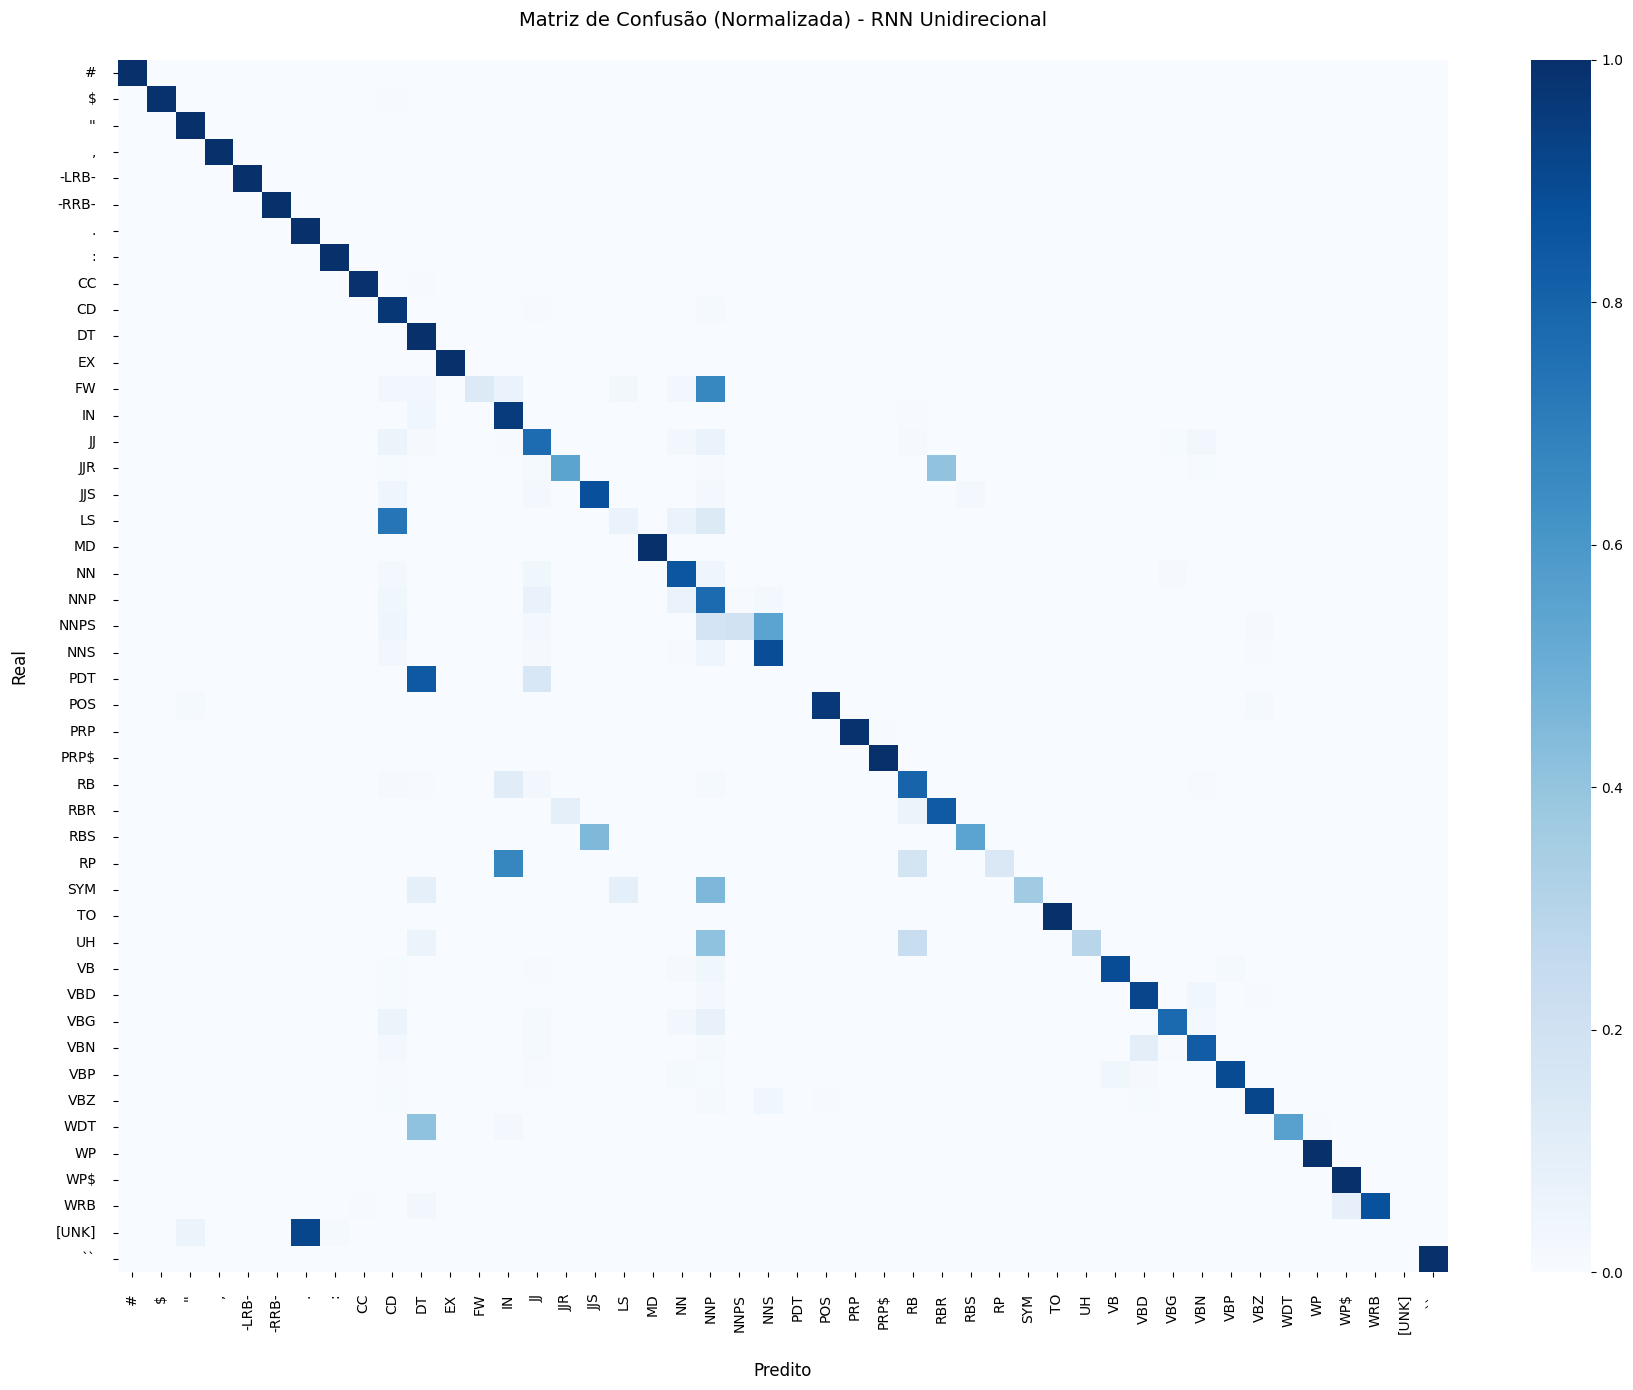
\includegraphics[width=\textwidth]{images/confusion_matrix/rnn_unidirecional.png}
        \caption{RNN Unidirecional}
        \label{fig:mx_simplernn_uni}
    \end{subfigure}
    \hfill
    \begin{subfigure}[b]{0.48\textwidth}
        \centering
        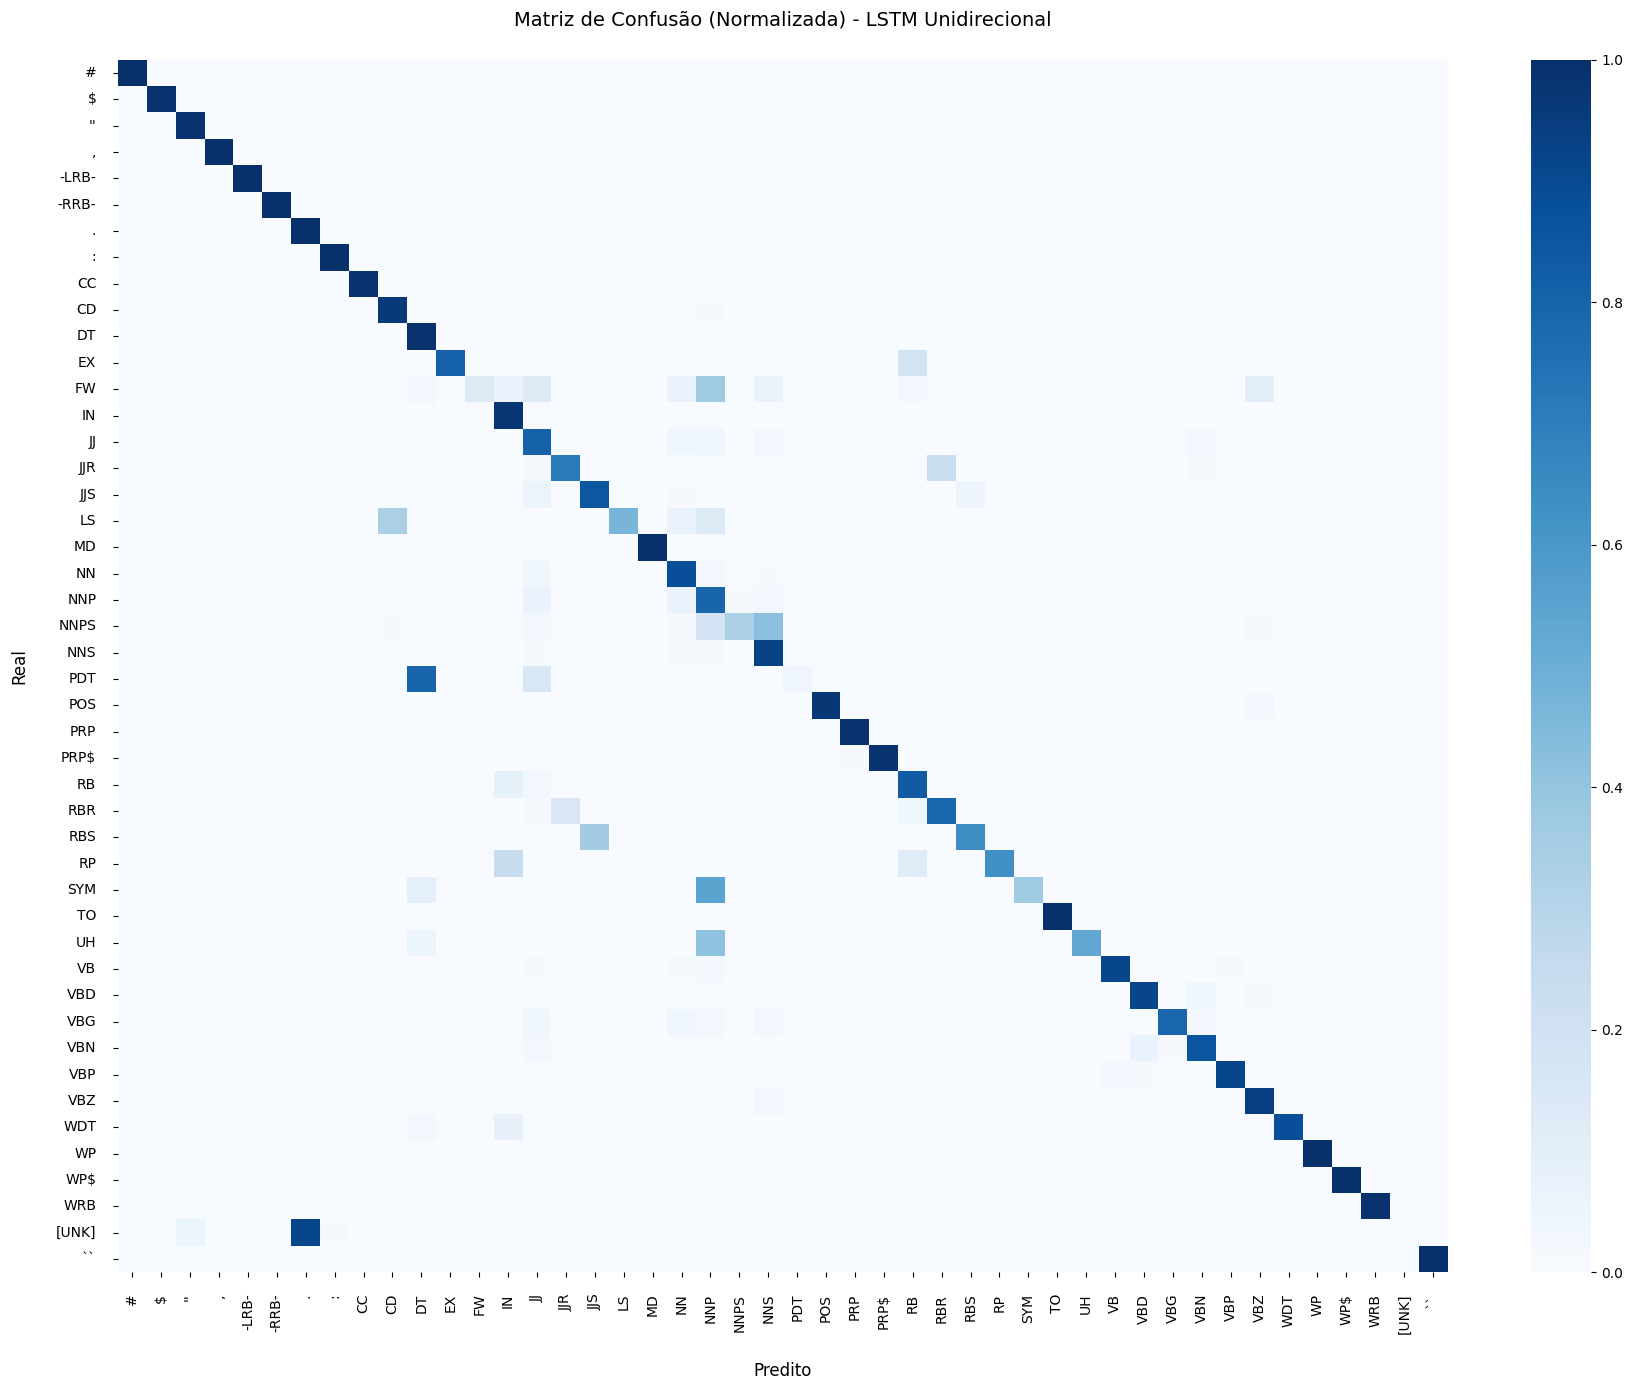
\includegraphics[width=\textwidth]{images/confusion_matrix/lstm_unidirecional.png}
        \caption{LSTM Unidirecional}
        \label{fig:mx_lstm_uni}
    \end{subfigure}

    \vspace{0.5cm}

    % Linha 2
    \begin{subfigure}[b]{0.48\textwidth}
        \centering
        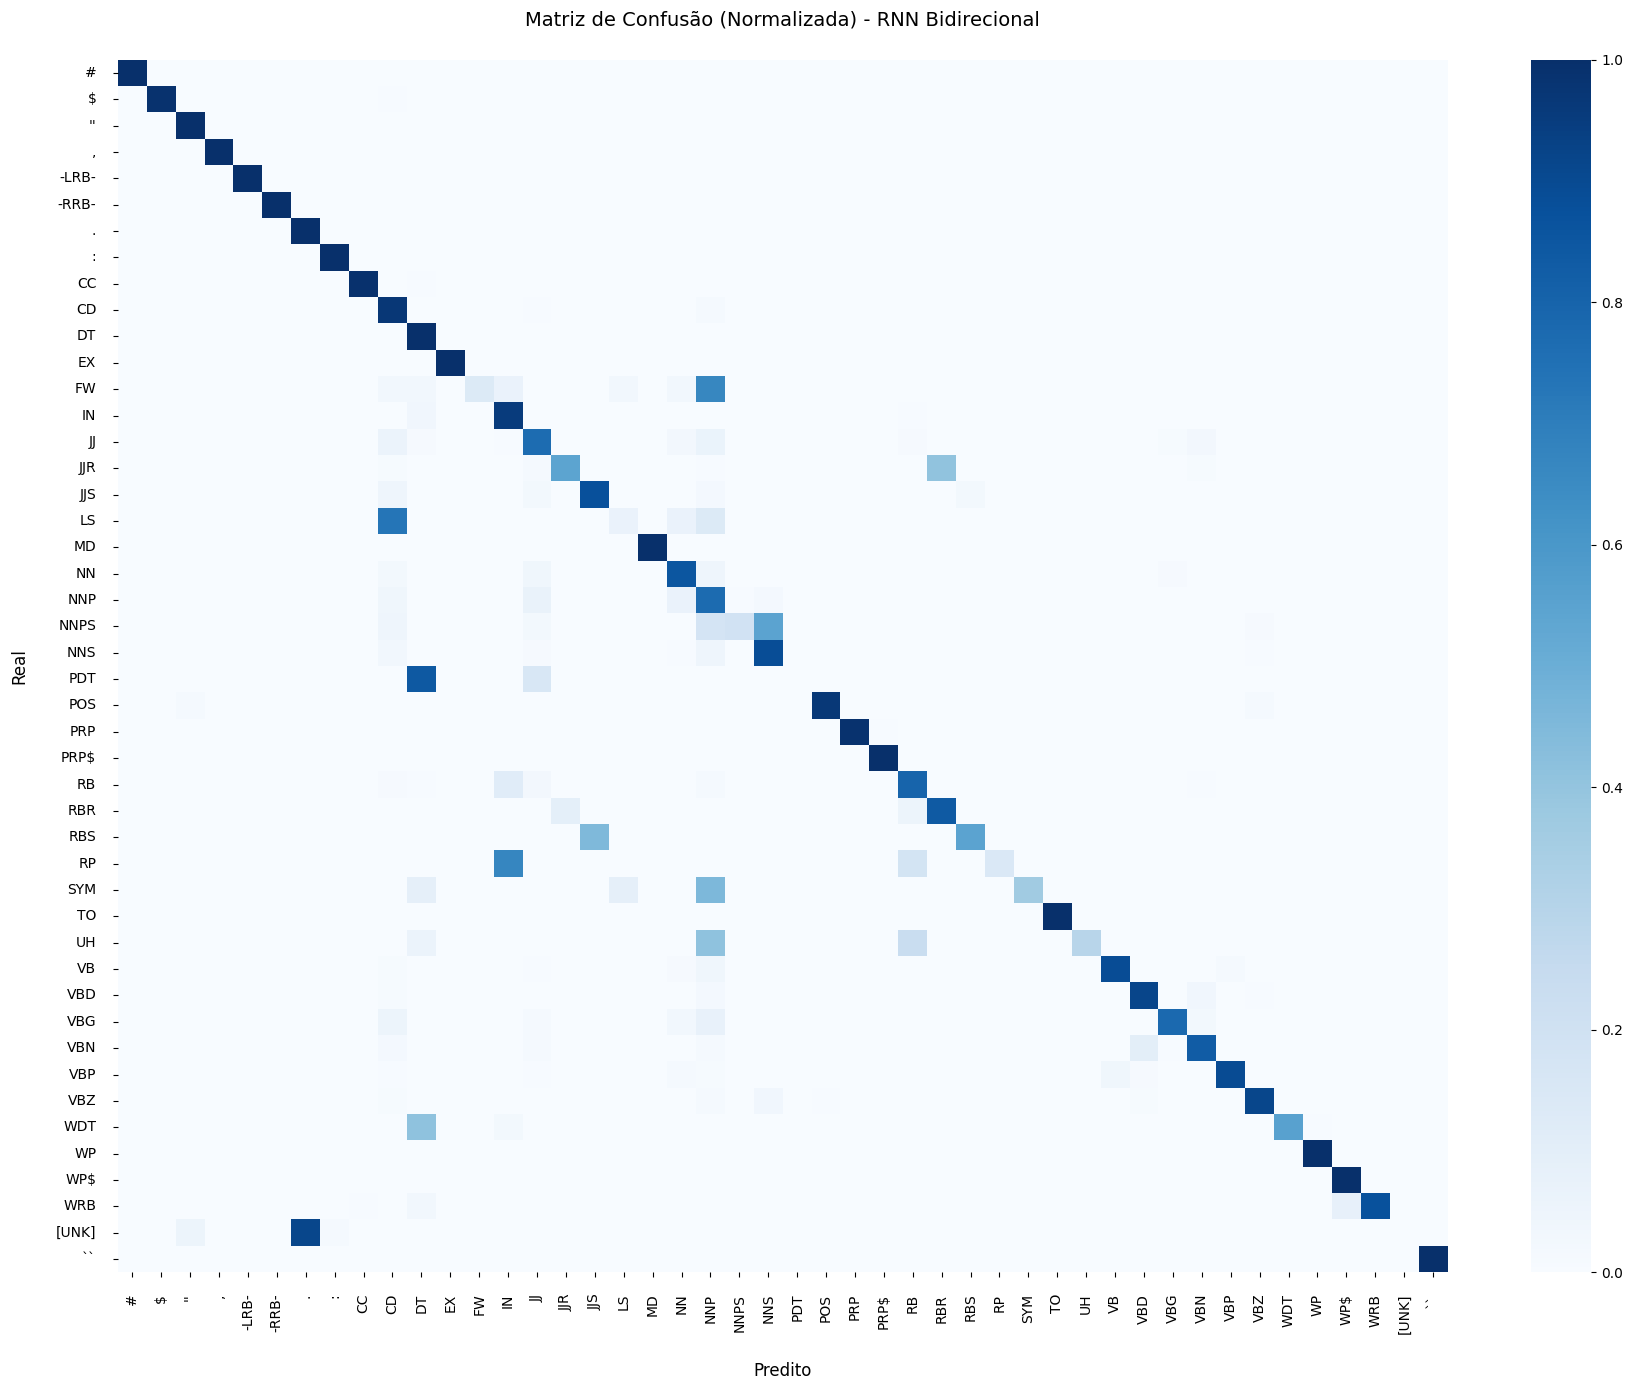
\includegraphics[width=\textwidth]{images/confusion_matrix/rnn_bidirecional.png}
        \caption{RNN Bidirecional}
        \label{fig:mx_simplernn_bi}
    \end{subfigure}
    \hfill
    \begin{subfigure}[b]{0.48\textwidth}
        \centering
        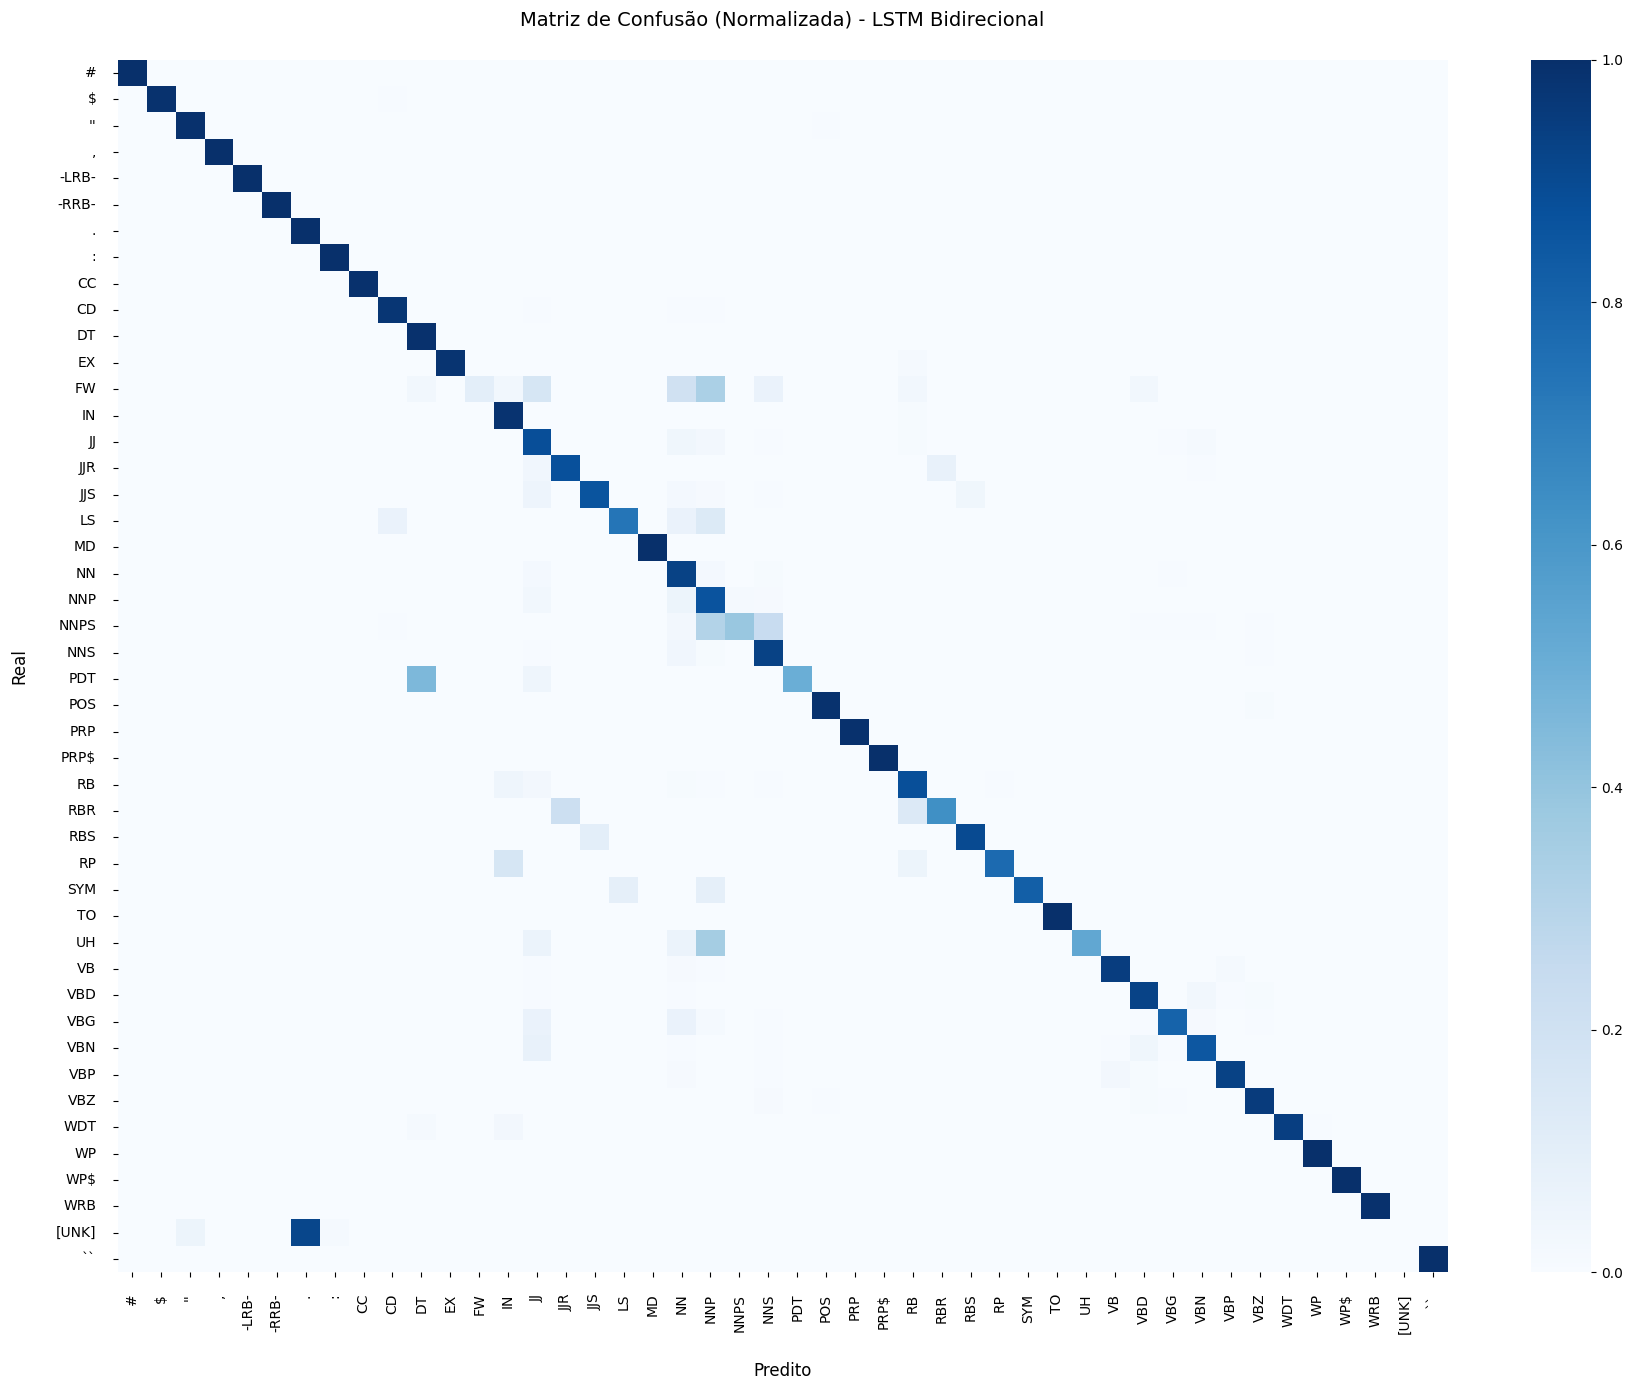
\includegraphics[width=\textwidth]{images/confusion_matrix/lstm_bidirecional.png}
        \caption{LSTM Bidirecional}
        \label{fig:mx_lstm_bi}
    \end{subfigure}

    \caption{Matrizes de Confusão obtidas no conjunto de teste para as quatro arquiteturas avaliadas.}
    \label{fig:matrizes_confusao_geral}
\end{figure}

Abaixo estão descritos os principais núcleos de desvio e confusão identificados no mapeamento:

\subsubsection*{O Núcleo de Ambiguidade Modificadora: JJ vs NN}
Um dos maiores focos de erro cruzado na matriz reside na fronteira entre \textbf{Adjetivos (\texttt{JJ})} e \textbf{Substantivos Comuns no Singular (\texttt{NN})}. Na língua inglesa, é extremamente comum que um substantivo atue temporariamente como um modificador adjunto de outro substantivo (como na expressão \textit{``crystal structure''}, onde \textit{crystal}, originalmente um substantivo, desempenha papel de adjetivo).
Os modelos unidirecionais sofrem para identificar essa transição devido à rigidez do fluxo sequencial, classificando incorretamente muitos adjetivos legítimos como substantivos. Nas redes bidirecionais, a precisão da classe \texttt{JJ} salta de 0,75 para 0,83 devido à capacidade de verificar se o token subsequente é um núcleo nominal.

\subsubsection*{O Problema de Capitalização de Entidades: NNP vs NN/NNPS}
A Matriz de Confusão evidencia um espessamento de erros na separação de \textbf{Substantivos Próprios (\texttt{NNP})} e Substantivos Comuns (\texttt{NN}), bem como entre suas respectivas formas plurais (\textbf{\texttt{NNPS}} vs. \textbf{\texttt{NNS}}).
Palavras raras ou não vistas pelo vocabulário que iniciam frases recebem o token de desconhecido (\texttt{[UNK]}). Por estarem capitalizadas na primeira letra devido à regra gramatical de início de período, as redes frequentemente confundem um substantivo comum de suporte sintático (\texttt{NN}) com um nome próprio (\texttt{NNP}).

A classe de substantivos próprios no plural (\texttt{NNPS}) obteve um dos piores desempenhos do relatório técnico (F1-score de apenas 0,27 na \textit{LSTM Bi}). A análise da matriz mostra que a rede majoritariamente desvia esses tokens para \texttt{NNP} (ignorando a flexão de número) ou para \texttt{NNS} (capturando o plural por causa do sufixo ``-s'', mas falhando em notar que se tratava de uma entidade própria devido ao suporte contextual fraco da frase).

\subsubsection*{Sufixos Verbais e Adjetivais: VBD vs VBN vs JJ}
Outro ponto crítico de confusão identificado na diagonal secundária envolve as tags de \textbf{Verbo no Passado (\texttt{VBD})}, \textbf{Verbo no Particípio (\texttt{VBN})} e \textbf{Adjetivos (\texttt{JJ})}.
Isso ocorre porque grande parte dos verbos regulares em inglês possuem exatamente a mesma terminação morfológica em ``-ed'' tanto para o passado simples quanto para o particípio (ex: \textit{``isolated''}). Além disso, o particípio pode atuar nativamente como um adjetivo predicativo (ex: \textit{``The patient felt isolated''}).

A matriz de confusão revela que os modelos unidirecionais tendem a classificar de forma enviesada a maioria dos tokens com terminação ``-ed'' como \texttt{VBD} por padrão estatístico de frequência. Novamente, a introdução das redes bidirecionais corrigiu esse desvio estrutural, permitindo que a rede olhasse se o token antecedente era um verbo auxiliar (como \textit{have/has} ou o verbo \textit{to be}), o que caracteriza matematicamente a ativação de um particípio (\texttt{VBN}) em detrimento de um passado simples.

\subsubsection*{Atenuação de Ruído e Contração da Dispersão: Unidirecionais vs Bidirecionais}
Ao contrastar visualmente as matrizes da Figura~\ref{fig:matrizes_confusao_geral}, nota-se uma nítida mudança no padrão de dispersão dos erros fora da diagonal principal. Nas matrizes das redes unidirecionais (\textit{RNN} e \textit{LSTM} Unidirecionais), há um espalhamento difuso de falsos positivos em colunas dominantes, o que indica que esses modelos recorrem a vieses de frequência estatística quando a palavra atual é ambígua.

Em contrapartida, as arquiteturas bidirecionais — especialmente a LSTM Bidirecional — demonstram uma contração drástica desse ruído periférico. O espessamento fora da diagonal principal é atenuado, confinando os erros estritamente aos pares linguísticos de altíssima ambiguidade (como os já discutidos \texttt{JJ} vs. \texttt{NN}).

No escopo dos métodos bidirecionais, a arquitetura de portas (\textit{gates}) da LSTM demonstrou superioridade analítica ao mitigar erros de classificação nos quais a \textit{SimpleRNN} bidirecional ainda falhava. Ao filtrar de maneira controlada as informações provenientes tanto do histórico quanto do contexto futuro da sequência, a LSTM foi capaz de eliminar falsas ativações em classes minoritárias, concentrando com maior precisão a densidade de probabilidade ao longo da diagonal principal da matriz de confusão.


\subsection{Transformer (Encoder-Only, Decoder-Only e Encoder-Decoder)}

\subsubsection{Estratégia de Implementação e Hiperparâmetros}
Os modelos baseados na arquitetura \textit{Transformer} foram construídos utilizando as bibliotecas \texttt{keras-nlp} e \texttt{keras-hub}. Todas as sentenças foram padronizadas para o mesmo comprimento com base no tamanho máximo do corpus. Para a representação das palavras, utilizou-se a matriz pré-treinada \textit{GloVe 6B} com 300 dimensões. As palavras ausentes no vocabulário original foram inicializadas aleatoriamente por meio de uma distribuição normal baseada na média e no desvio padrão dos vetores do GloVe.

O treinamento de todas as variantes utilizou o otimizador \textit{AdamW} (com taxa de aprendizado inicial fixada em $0,001$) e a função de perda \textit{Sparse Categorical Crossentropy}. Aplicou-se o critério de parada prematura (\textit{EarlyStopping}) com base na métrica customizada \texttt{MaskedAccuracy}, configurando uma tolerância de até 3 épocas e recuperando os melhores pesos obtidos. Essa métrica de acurácia foi desenvolvida para desconsiderar os tokens de preenchimento (\texttt{[PAD]}), marcas de início (\texttt{[START]}), termos desconhecidos (\texttt{[UNK]}) e os símbolos de pontuação do \textit{Penn Treebank}.

As três variações possuem as seguintes especificações estruturais:
\begin{itemize}
    \item \textbf{Transformer Encoder-Only:} Contém 2 blocos de \texttt{TransformerEncoder}, dimensão intermediária (camada feed-forward) de 256, 4 cabeças de atenção e taxa de \textit{dropout} de 0,3 no primeiro bloco e 0,2 no segundo. A classificação é feita por uma camada linear final com ativação \textit{softmax} (Total de 5.621.959 parâmetros).
    \item \textbf{Transformer Decoder-Only:} Composto por 1 bloco de \texttt{TransformerDecoder} com máscara causal, dimensão intermediária de 256, 4 cabeças de atenção e \textit{dropout} de 0,2. A classificação também ocorre por meio de uma camada linear com \textit{softmax} (Total de 5.105.403 parâmetros).
    \item \textbf{Transformer Encoder-Decoder:} O \textit{Encoder} processa a sentença com embeddings de 300 dimensões e o \textit{Decoder} gera as tags com auxílio de mecanismo de \textit{Cross-Attention}. Durante o treino, aplicou-se a técnica de \textit{Teacher Forcing} utilizando uma camada de embedding exclusiva para as tags com 64 dimensões (Total de 5.210.344 parâmetros).
\end{itemize}

\subsubsection{Resultados Gerais e Análise de Performance}
Os modelos foram avaliados no conjunto de validação do corpus, e as acurácias obtidas estão apresentadas na Tabela~\ref{tab:resultados_transformers}:

\begin{table}[H]
\centering
\begin{tabular}{|l|c|c|}
\hline
\textbf{Modelo/Arquitetura} & \textbf{Acurácia Mascarada} & \textbf{Total de Parâmetros Treináveis} \\ \hline
Transformer Decoder-Only    & 92,77\%                     & 5.105.403                             \\ \hline
Transformer Encoder-Only    & 93,93\%                     & 5.621.959                             \\ \hline
Transformer Encoder-Decoder & 94,40\%                     & 5.210.344                             \\ \hline
\end{tabular}
\caption{Desempenho dos modelos Transformer na tarefa de POS Tagging.}
\label{tab:resultados_transformers}
\end{table}

Os dados indicam que o modelo \textbf{Encoder-Decoder} obteve o maior índice de acerto (94,40\%), seguido pelo \textit{Encoder-Only} (93,93\%). Uma provável explicação para a diferença a favor do Encoder-Decoder é o uso de um espaço de embedding menor e separado para as tags (64d), o que pode ter simplificado a modelagem da sequência de saída pelo Decoder, mantendo a consulta livre ao texto original via atenção cruzada.

O modelo \textbf{Decoder-Only} apresentou o menor resultado (92,77\%). Esse comportamento reflete o impacto da máscara causal, que impede o modelo de acessar as palavras localizadas à direita do token atual durante o processamento. Como a classificação gramatical em inglês frequentemente depende de termos subsequentes (como substantivos posicionados após adjetivos), a falta desse contexto reduz o desempenho geral do modelo.

\subsubsection{Análise das Matrizes de Confusão}

\begin{figure}[htbp]
    \centering
    % Linha 1
    \begin{subfigure}[b]{0.48\textwidth}
        \centering
        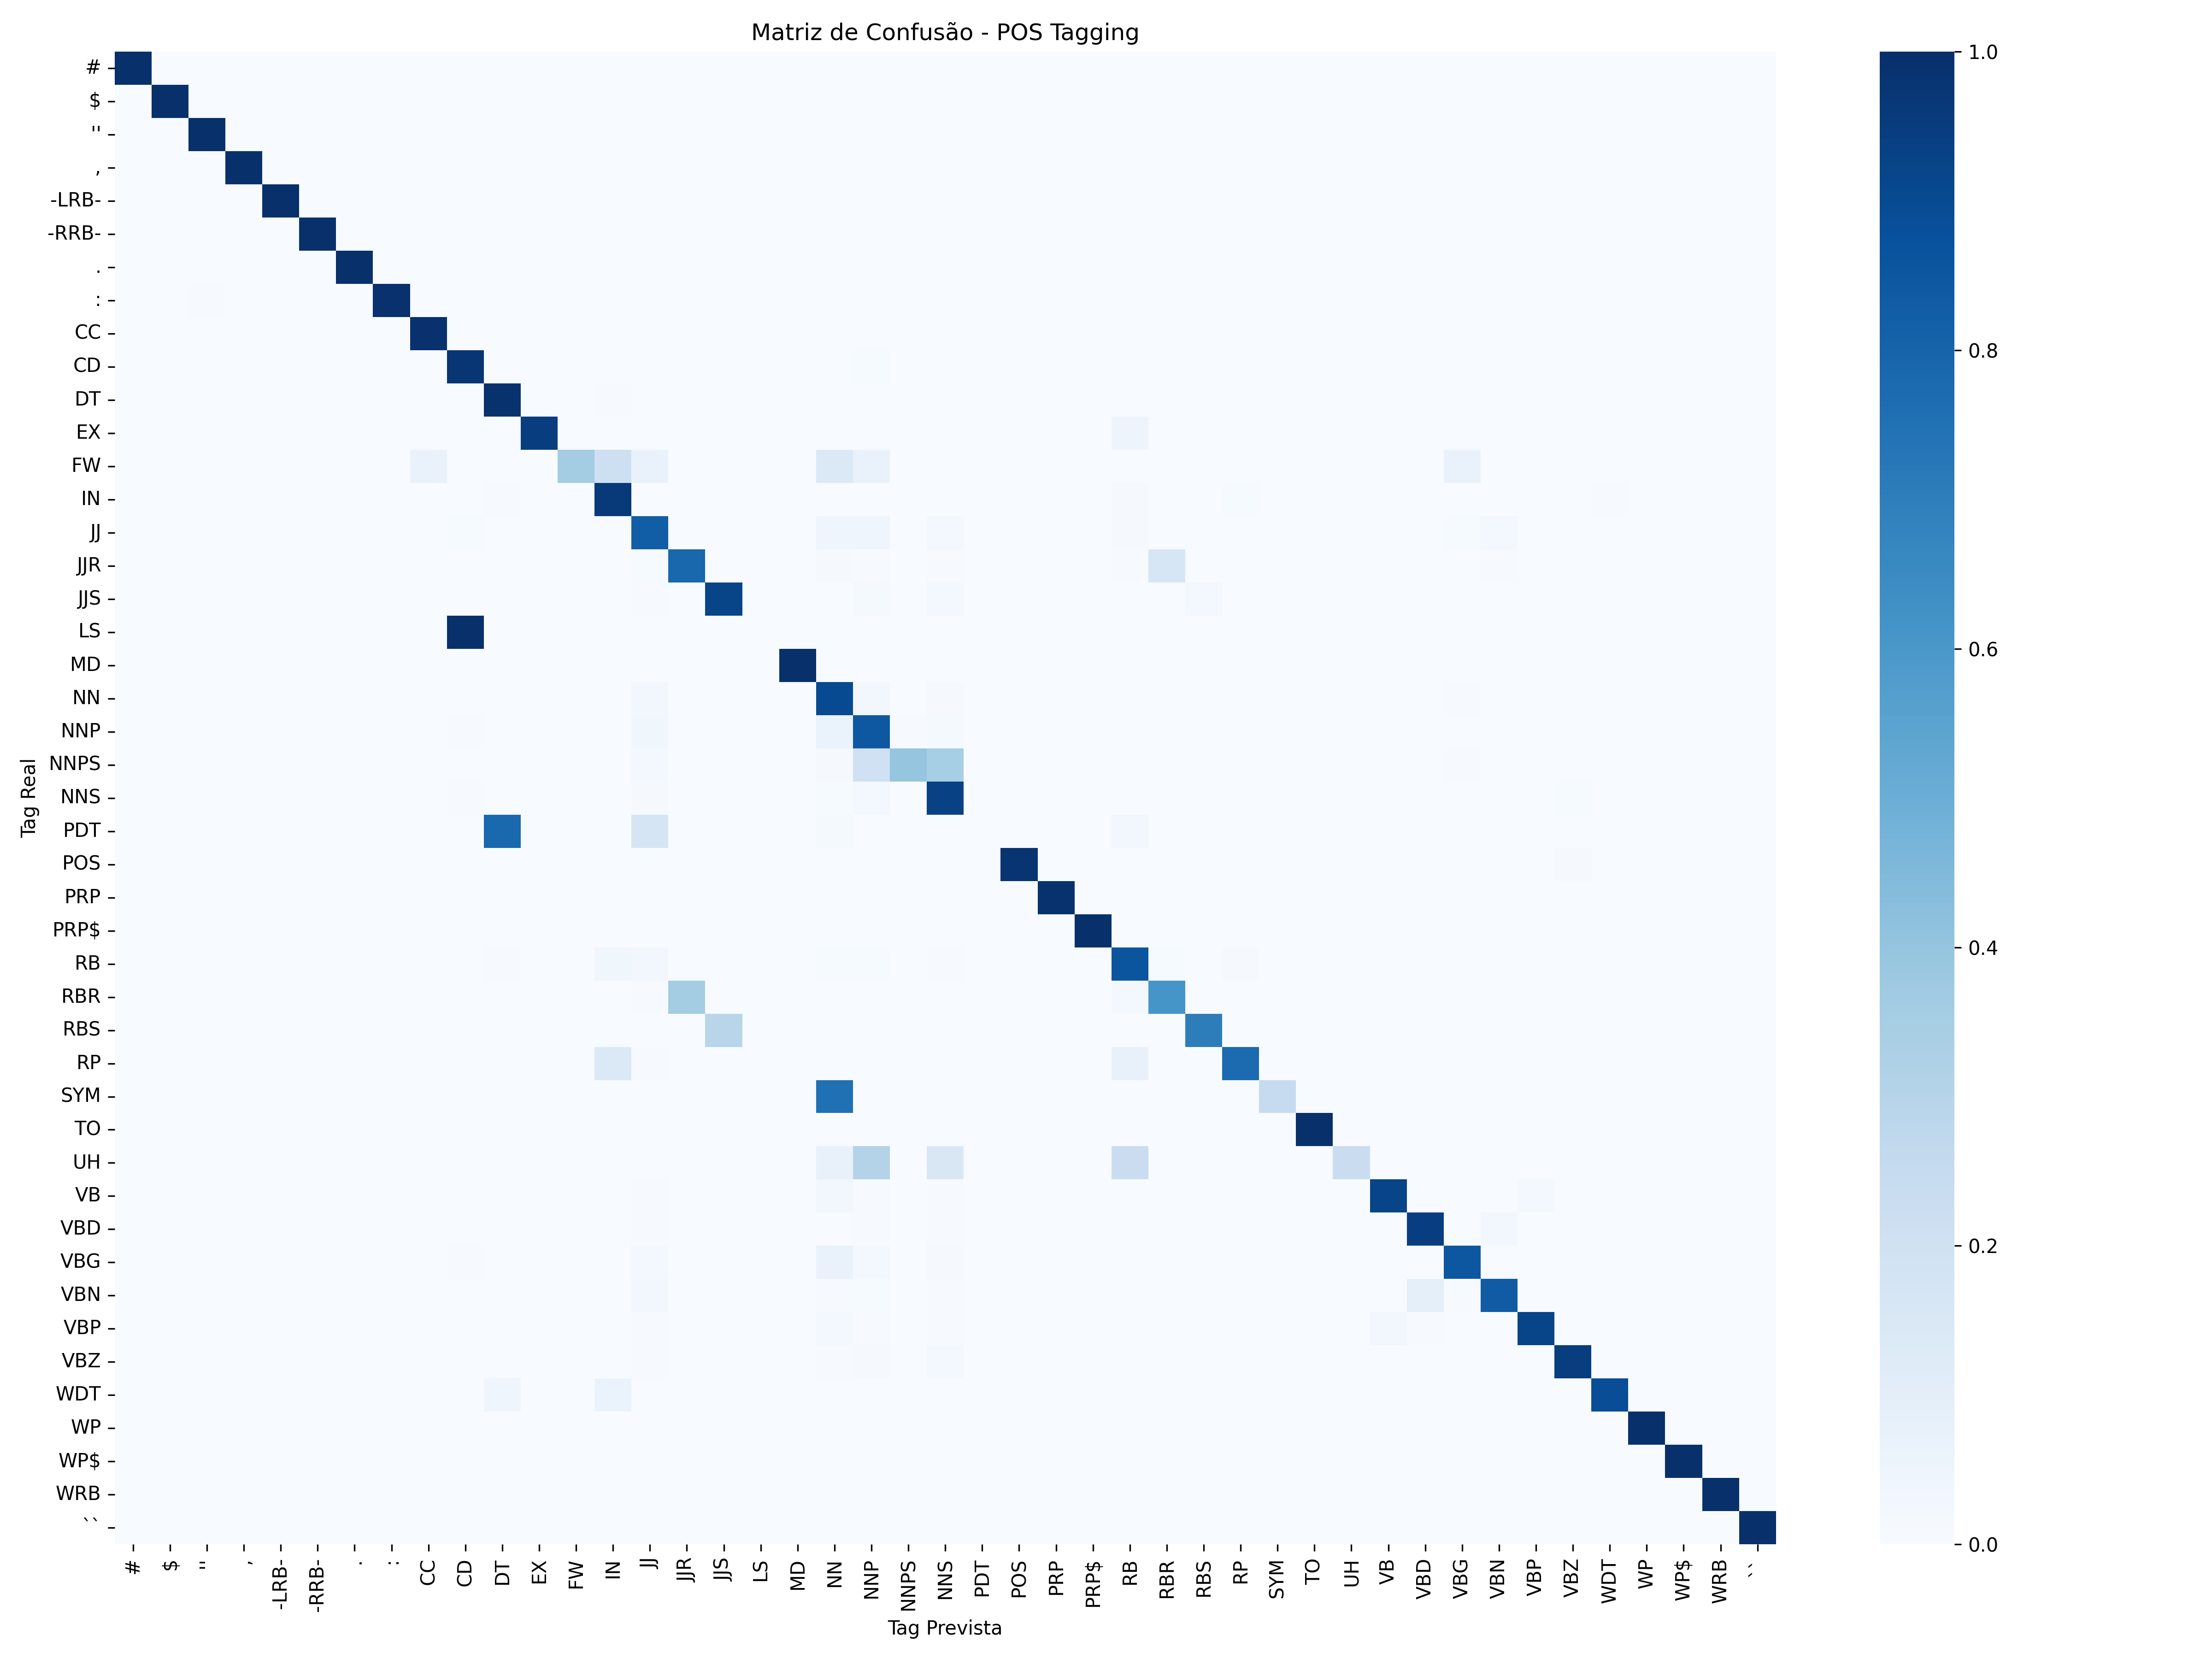
\includegraphics[width=\textwidth]{images/confusion_matrix/decoder.png}
        \caption{Decoder-Only}
        \label{fig:mx_decoder}
    \end{subfigure}
    \hfill
    \begin{subfigure}[b]{0.48\textwidth}
        \centering
        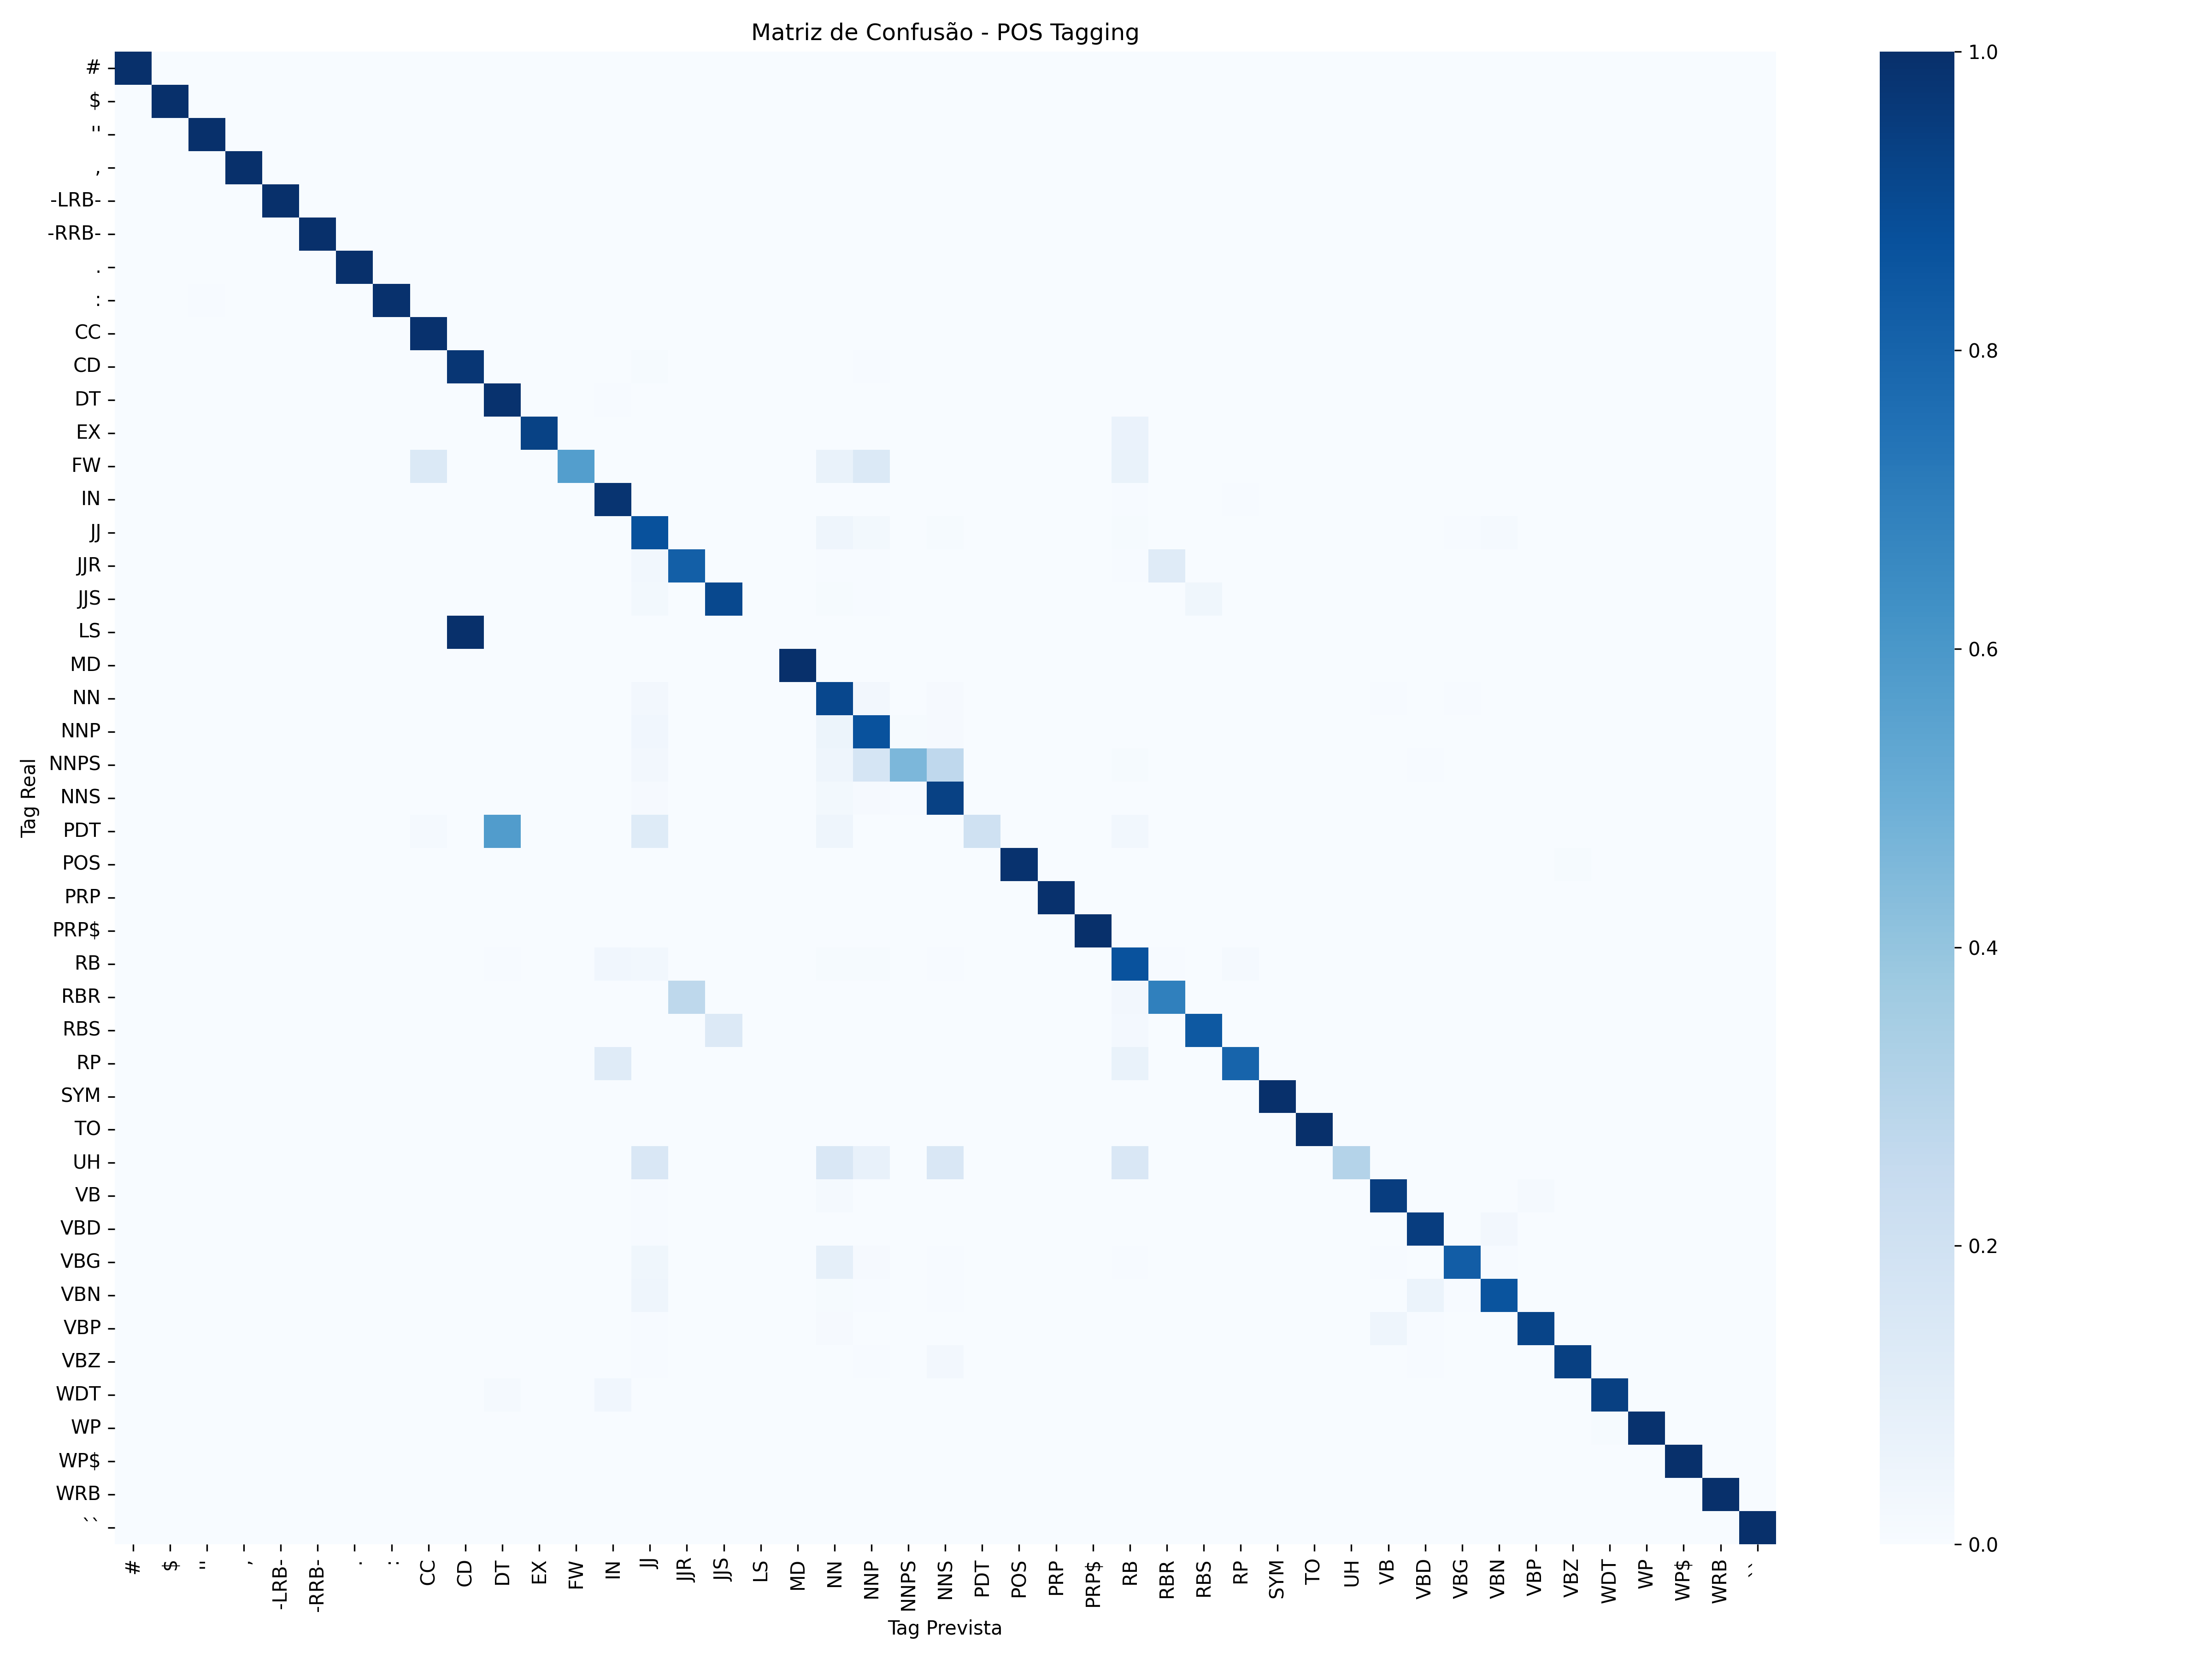
\includegraphics[width=\textwidth]{images/confusion_matrix/encoder.png}
        \caption{Encoder-Only}
        \label{fig:mx_encoder}
    \end{subfigure}

    \vspace{0.5cm}

    % Linha 2
    \begin{subfigure}[b]{0.48\textwidth}
        \centering
        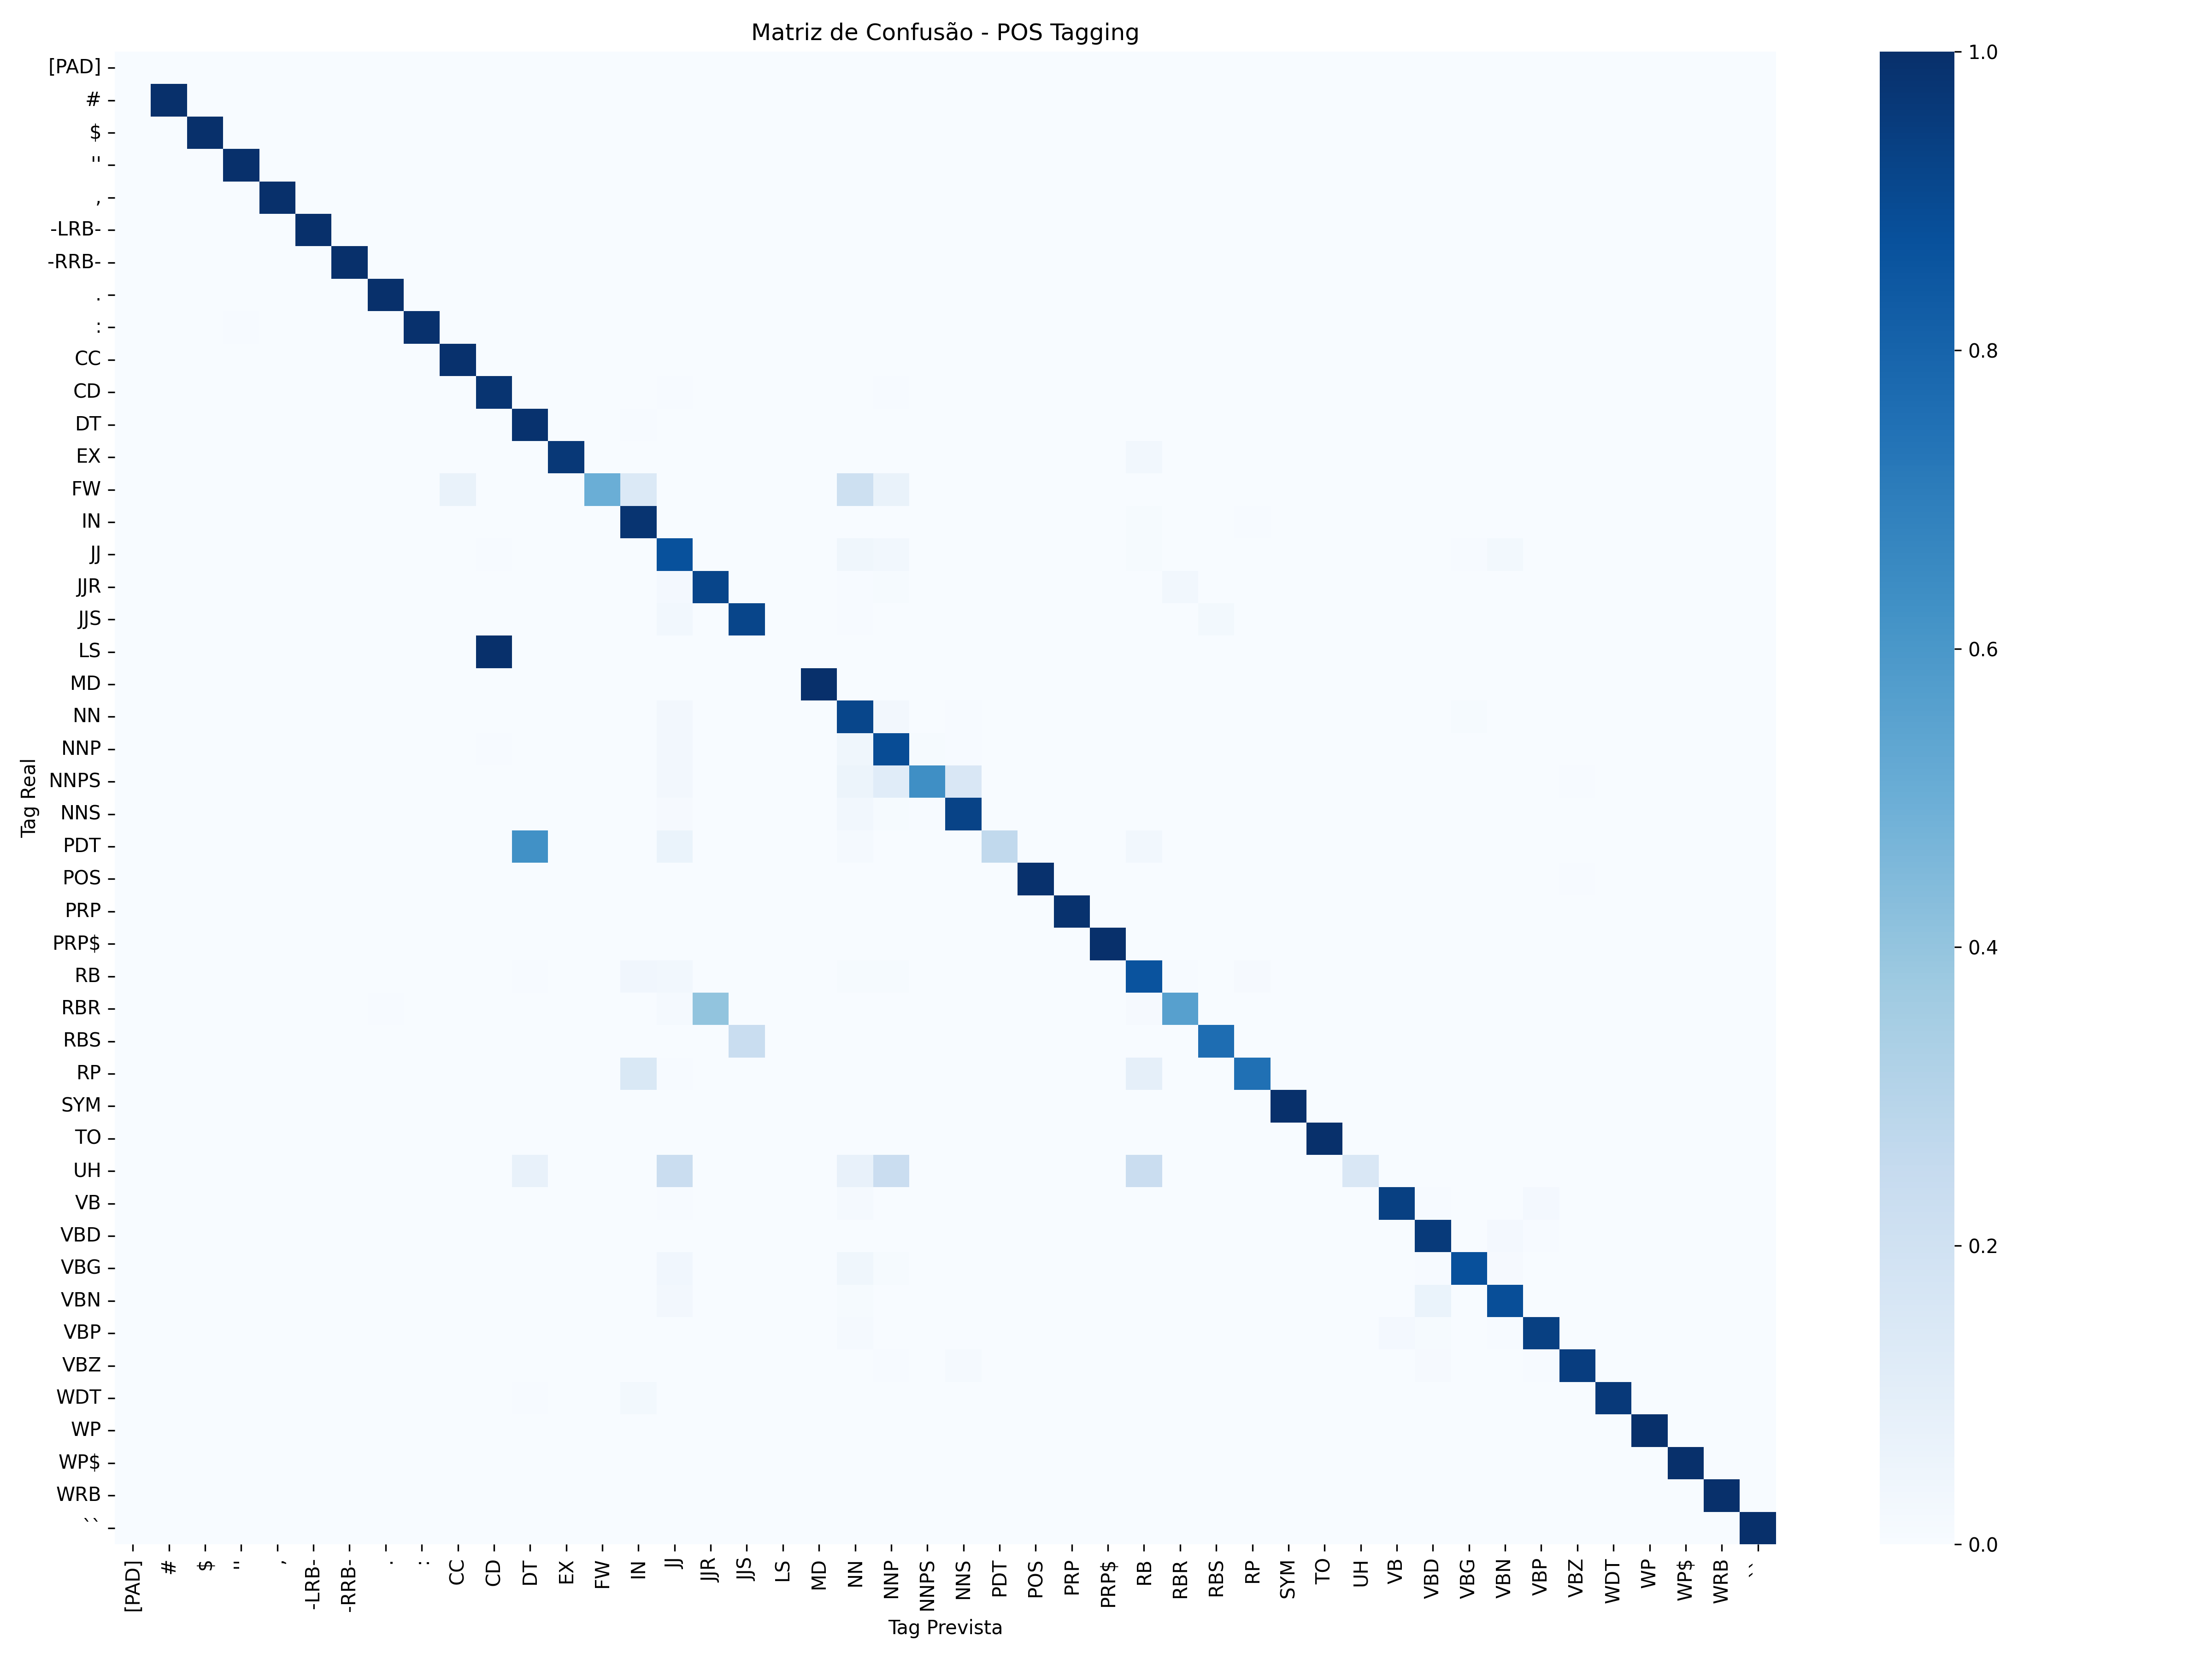
\includegraphics[width=\textwidth]{images/confusion_matrix/encoder_decoder.png}
        \caption{Encoder-Decoder}
        \label{fig:mx_enc_dec}
    \end{subfigure}
    \hfill

    \caption{Matrizes de Confusão obtidas no conjunto de validação para as arquiteturas baseadas em Transformer.}
    \label{fig:matrizes_confusion_transformers}
\end{figure}

Na matriz do modelo \textit{Encoder-Only}, observa-se que os erros se concentram em classes com forte semelhança morfológica. Ocorre uma confusão recorrente entre substantivos próprios no plural (\texttt{NNPS}) e substantivos comuns no plural (\texttt{NNS}). Outro ponto de desvio aparece na tag \texttt{LS} (\textit{List item marker}), que é algumas vezes classificada como determinante (\texttt{DT}), possivelmente por sua posição isolada no início dos períodos textuais.

A análise do modelo \textit{Decoder-Only} mostra uma dispersão maior de erros fora da diagonal principal, principalmente nas linhas correspondentes a adjetivos (\texttt{JJ}) e advérbios (\texttt{RB}). Devido à restrição de não visualizar o contexto futuro, o modelo exibe maior dificuldade para discernir essas classes em comparação com os modelos não-causais.

O mapa de calor do modelo \textit{Encoder-Decoder} apresenta uma concentração de acertos mais limpa na diagonal principal. Contudo, há um desvio perceptível entre os tempos verbais no passado simples (\texttt{VBD}) e no particípio (\texttt{VBN}). Esse erro pode estar associado à natureza autorregressiva do decodificador, onde a predição incorreta de uma tag inicial pode influenciar a classificação dos elementos vizinhos na sequência.


\newpage
\subsection{Tagging usando uma LLM Comercial via API}

\subsubsection{Metodologia}

Inicialmente foi realizado um pré-processamento dos dados para posterior utilização. O pipeline de preparação dos dados verifica a consistência do tagset entre as três divisões do banco (treino, validação e teste) e detecta sentenças duplicadas entre elas. Tokens com a tag -NONE-, que não correspondem a palavras de superfície, são removidos nessa etapa.

O código foi organizado em módulos com diferentes responsabilidades:

\begin{itemize}
    \item \textbf{prepare\_ptb\_splits.py:} parsing dos três arquivos fonte e geração dos conjuntos data/train.json, data/val.json e data/test.json em um schema JSON uniforme;
    \item \textbf{prompts.py:} templates de prompt para todos os modos;
    \item \textbf{retrieval.py:} índice  de recuperação para o RAG(Retrieval-Augmented-Generation), baseado em TF-IDF e similaridade de cosseno sobre o pool de treino;
    \item \textbf{ai\_client.py:} wrapper de chamada à API do modelo de linguagem, com parsing e validação de saída e retentativas em caso de formato inválido;
    \item \textbf{run\_tagging.py:} orquestra a execução de um modo sobre um split, salvando os resultados;
    \item \textbf{evaluate.py:} calcula a acurácia por token, gera o relatório de classificação por tag e a matriz de confusão, além de comparar os três modos.
\end{itemize}

\subsubsection{Estratégias Implementadas e Avaliações}

Em todos os modos, o modelo recebe instruções fixas de sistema especificando o tagset completo do Penn Treebank e exigindo que a resposta seja exclusivamente um array JSON de tags, na mesma ordem e quantidade dos tokens de entrada, sem re-tokenizar a sentença. Essa restrição de formato foi adotada para evitar o problema clássico de alinhamento entre a tokenização da entrada e a saída gerada pelo modelo. Os três métodos implementados foram os seguintes:

\begin{itemize}
    \item \textbf{Zero-shot:} O prompt contém apenas as instruções de sistema e a sentença a ser tageada. O modelo depende inteiramente do conhecimento adquirido no pré-treinamento;
    \item \textbf{Few-Shot:} O prompt inclui, além das instruções, um conjunto fixo de 5 exemplos rotulados, escolhidos manualmente uma única vez e reutilizados para todas as sentenças de teste, independentemente do seu conteúdo;
    \item \textbf{RAG:} Para cada sentença de teste, um índice TF-IDF sobre as 38 mil sentenças do pool de treino é consultado para recuperar as 5 sentenças mais similares por similaridade de cosseno, que então compõem os exemplos do prompt daquela sentença específica.
\end{itemize}

A métrica principal é a acurácia por token, ou seja, a proporção de tokens cuja tag predita coincide com o que está avaliado no PTB. Sentenças em que o modelo não retornou um JSON válido, ou retornou uma quantidade de tags diferente da quantidade de tokens de entrada, são registradas separadamente como falha de geração e excluídas do cálculo de acurácia, essa escolha metodológica que evita que erros de formatação se confundam com erros de classificação linguística propriamente ditos.

\begin{longtable}[c]{|c|c|c|c|c|}
\hline
\textbf{Modo} & \textbf{Acurácia} & \textbf{Tokens Avaliados} & \textbf{Sentenças c/ falha} & \textbf{IC 95\% (Wilson)} \\
\hline
Zero-shot & 91,75\% & 1.879 & 15/100 & [90,42\%; 92,91\%]. \\
\hline
Few-shot & 93,91\% & 1.971 & 11/100 & [92,77\%; 94,88\%]. \\
\hline
RAG & 94,39\% & 1.853 & 14/100 & [93,24\%; 95,35\%]. \\
\hline
\caption{Avaliação dos métodos implementados}
\end{longtable}

O número de tokens avaliados difere entre os três modos mesmo partindo das mesmas 100 sentenças: como sentenças com falha de geração são descartadas do cálculo, e cada modo falhou em sentenças diferentes, cada acurácia foi calculada sobre um subconjunto de tokens ligeiramente distinto. Segundo, ao considerar os intervalos de confiança, o intervalo do zero-shot ([90,42\%; 92,91\%]) e o do few-shot ([92,77\%; 94,88\%]) praticamente não se sobrepõem, sugerindo uma diferença real entre as duas condições. Já os intervalos do few-shot e do RAG se sobrepõem substancialmente, o que indica que a diferença de 0,48 ponto percentual entre eles não é estatisticamente robusta nessa amostra de 100 sentenças.

Além da acurácia, a proporção de sentenças em que o modelo não produziu uma saída bem formada é, por si só, um resultado relevante: zero-shot falhou em 15\% das sentenças, few-shot em 11\% e RAG em 14\%. O padrão geral, falhas mais frequentes sem exemplos do que com exemplos, é consistente com a hipótese de que demonstrações no prompt ajudam o modelo a aderir ao formato de saída solicitado, uma função que Min et al. (2022) atribuem aos exemplos independentemente da correção de seus rótulos. O RAG ter uma taxa de falha discretamente maior que o few-shot estático, apesar de exemplos tematicamente mais relevantes, é compatível com a possibilidade de que as sentenças recuperadas por similaridade tendam a ser mais longas ou sintaticamente mais complexas que os exemplos fixos, tornando o prompt como um todo mais difícil de ser seguido.

\subsubsection{Matriz de Confusão}

As matrizes de confusão normalizadas mostram, para cada modo, a proporção de cada tag real classificada como cada tag predita. Em todos os três modos a diagonal principal concentra a maior parte da massa, como esperado, a maioria das tags é classificada corretamente pelo LLM mesmo sem qualquer ajuste fino.

\begin{figure}[H]
    \centering
    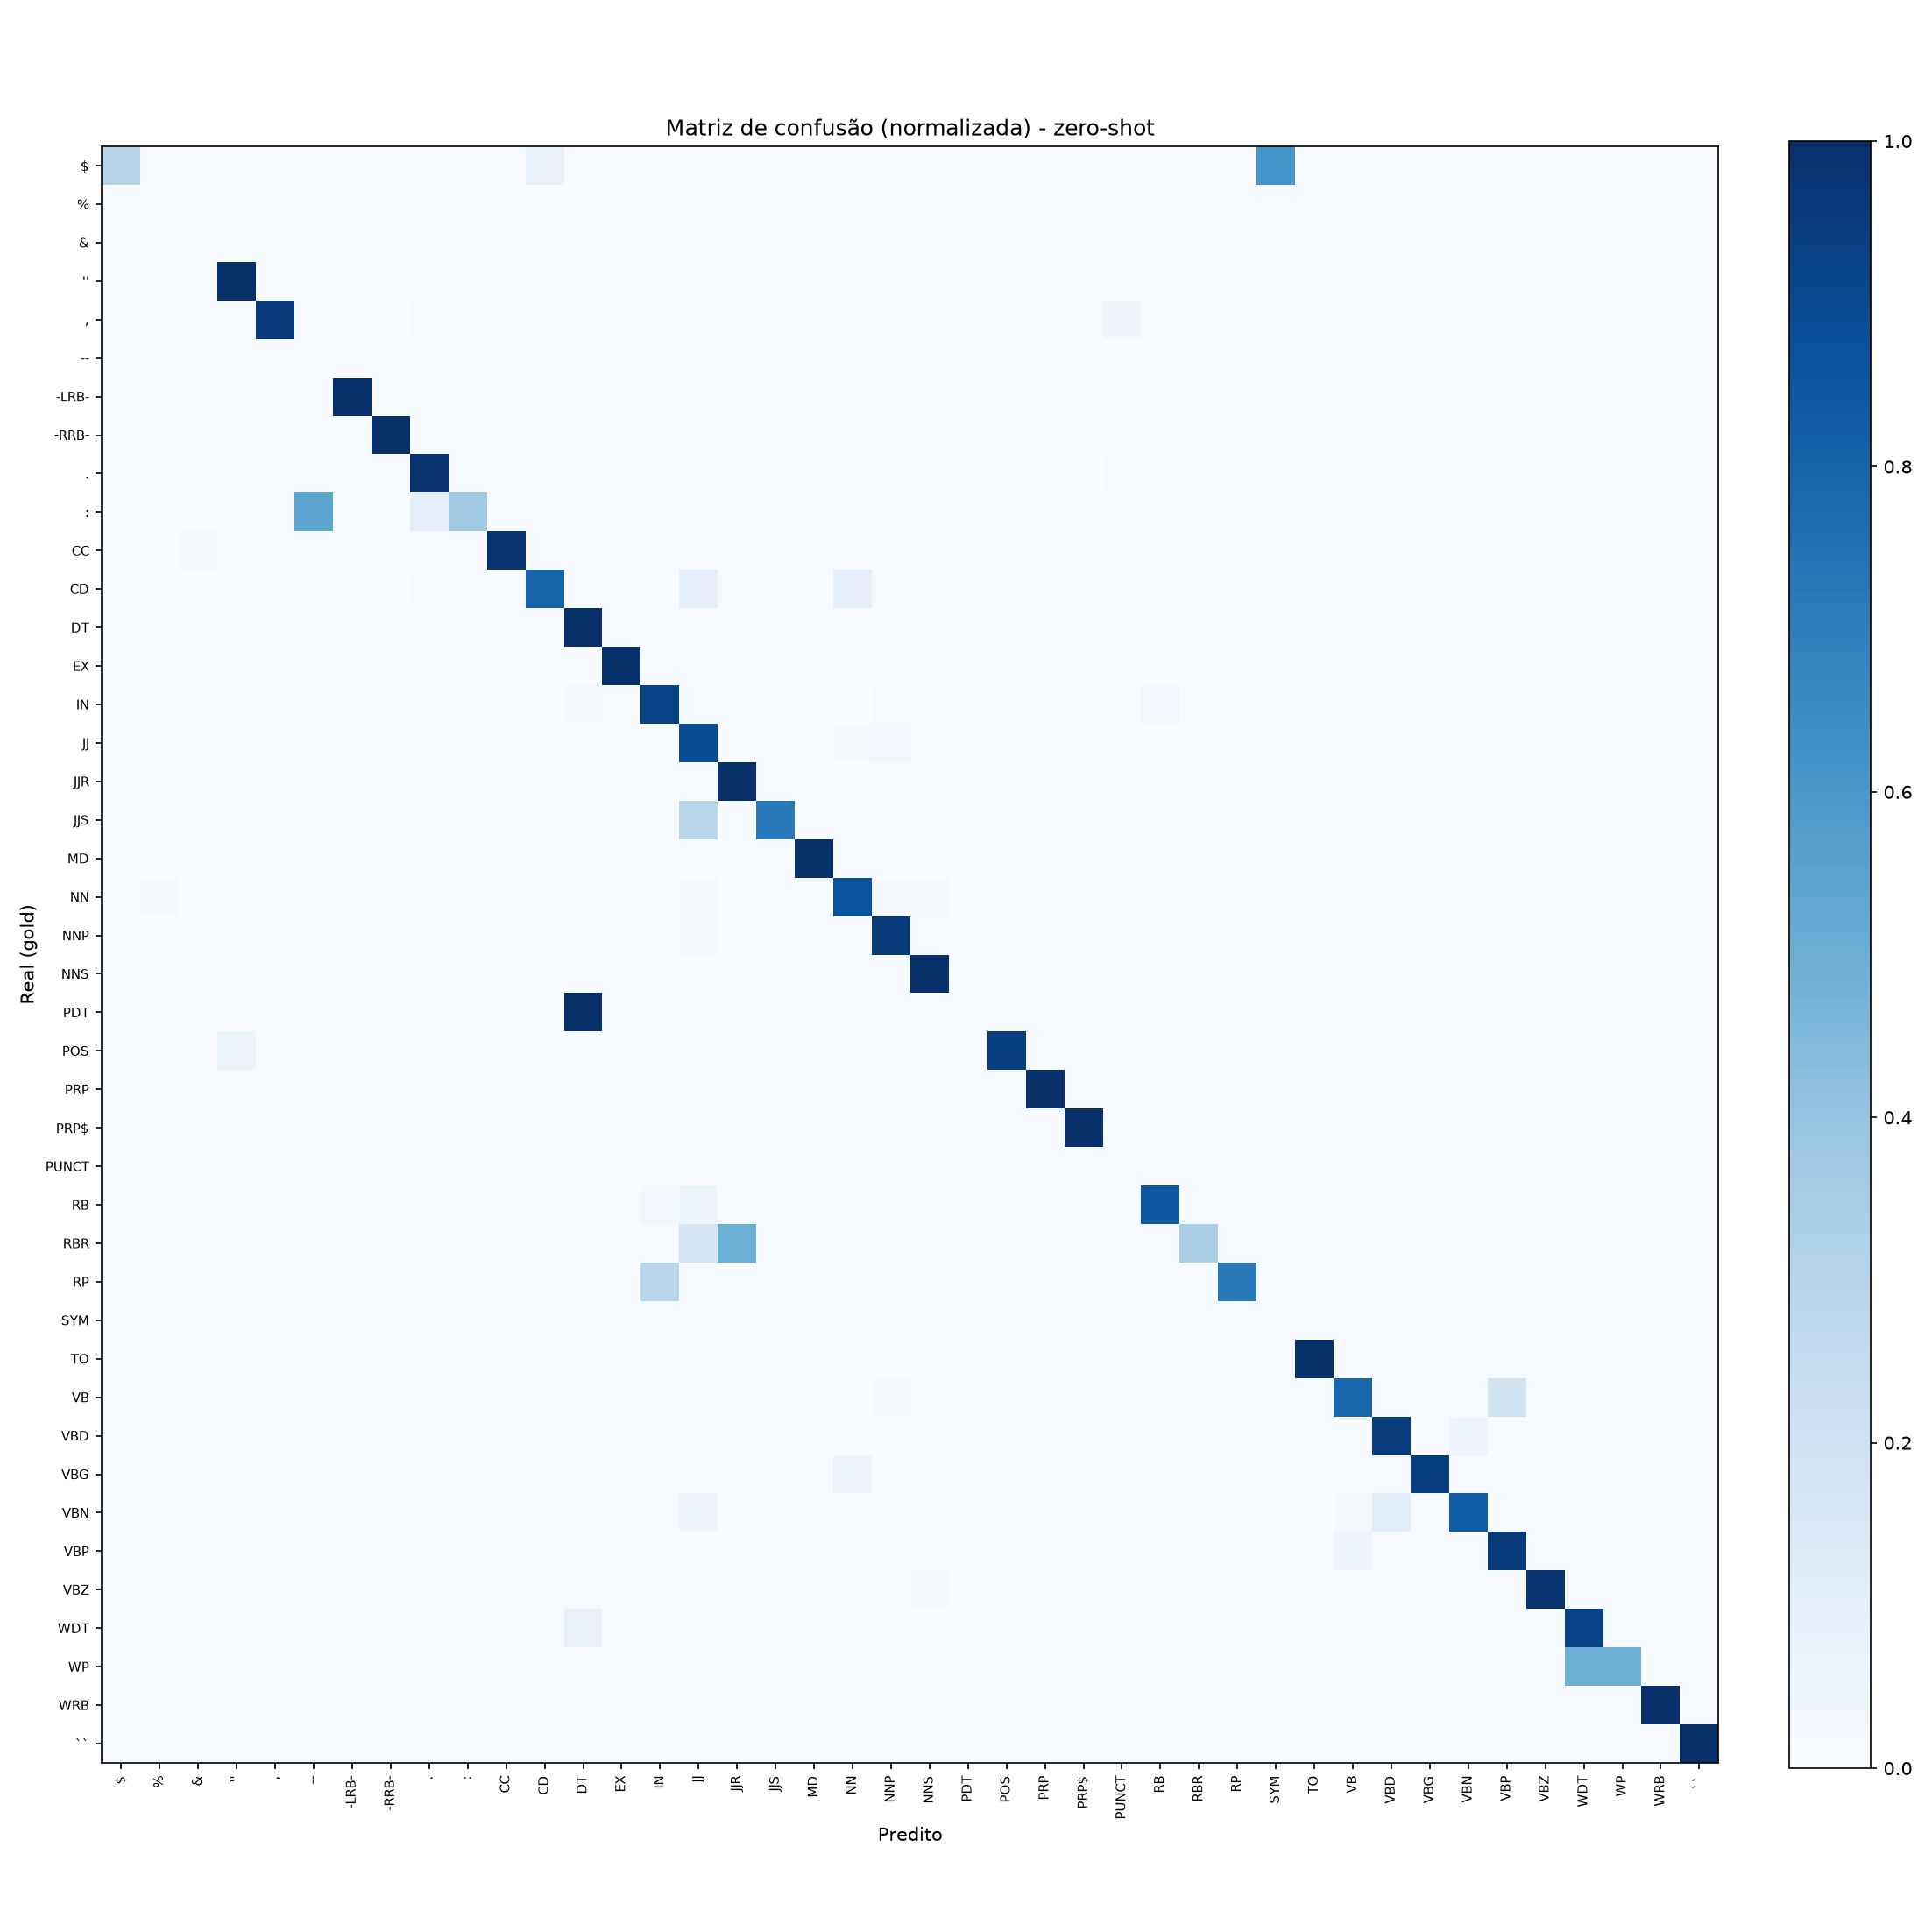
\includegraphics[width=0.9\textwidth]{images/confusion_matrix/zero-shot.png}
    \caption{Matriz de Confusão do zero-shot.}
    \label{fig:zero_shot}
\end{figure}

\begin{figure}[H]
    \centering
    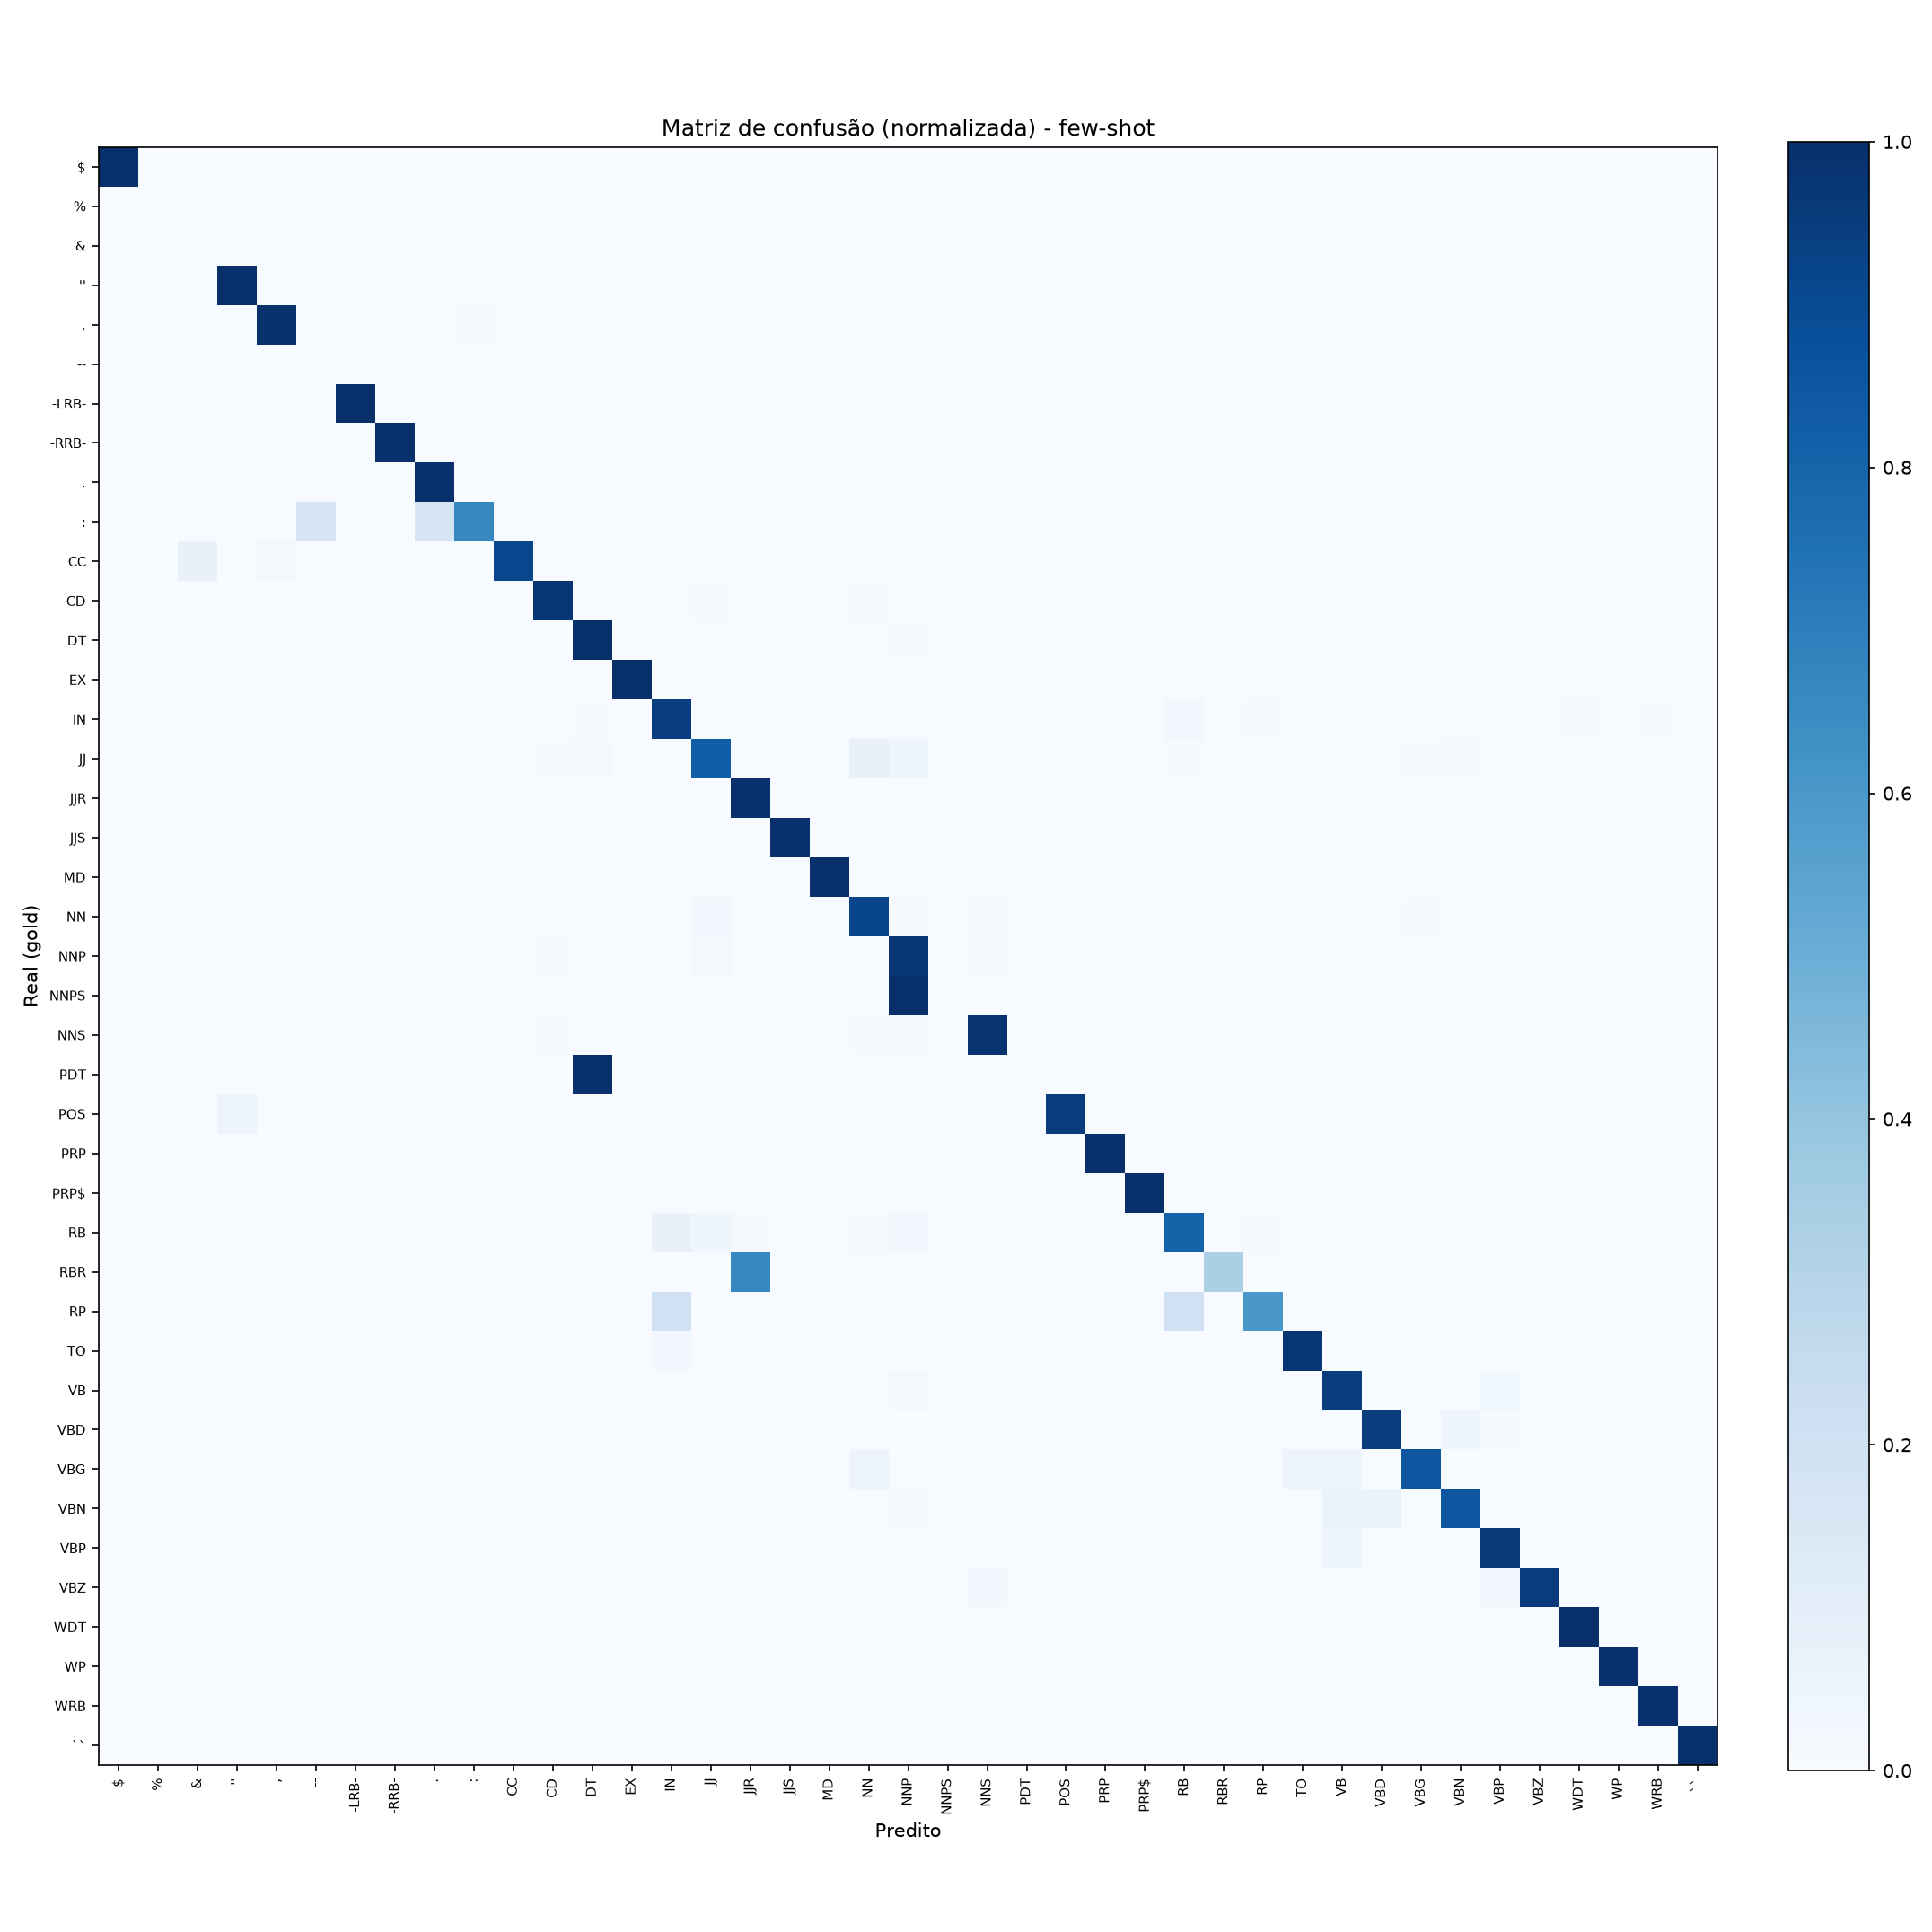
\includegraphics[width=0.9\textwidth]{images/confusion_matrix/few-shot.png}
    \caption{Matriz de Confusão do few-shot.}
    \label{fig:few_shot}
\end{figure}

\begin{figure}[H]
    \centering
    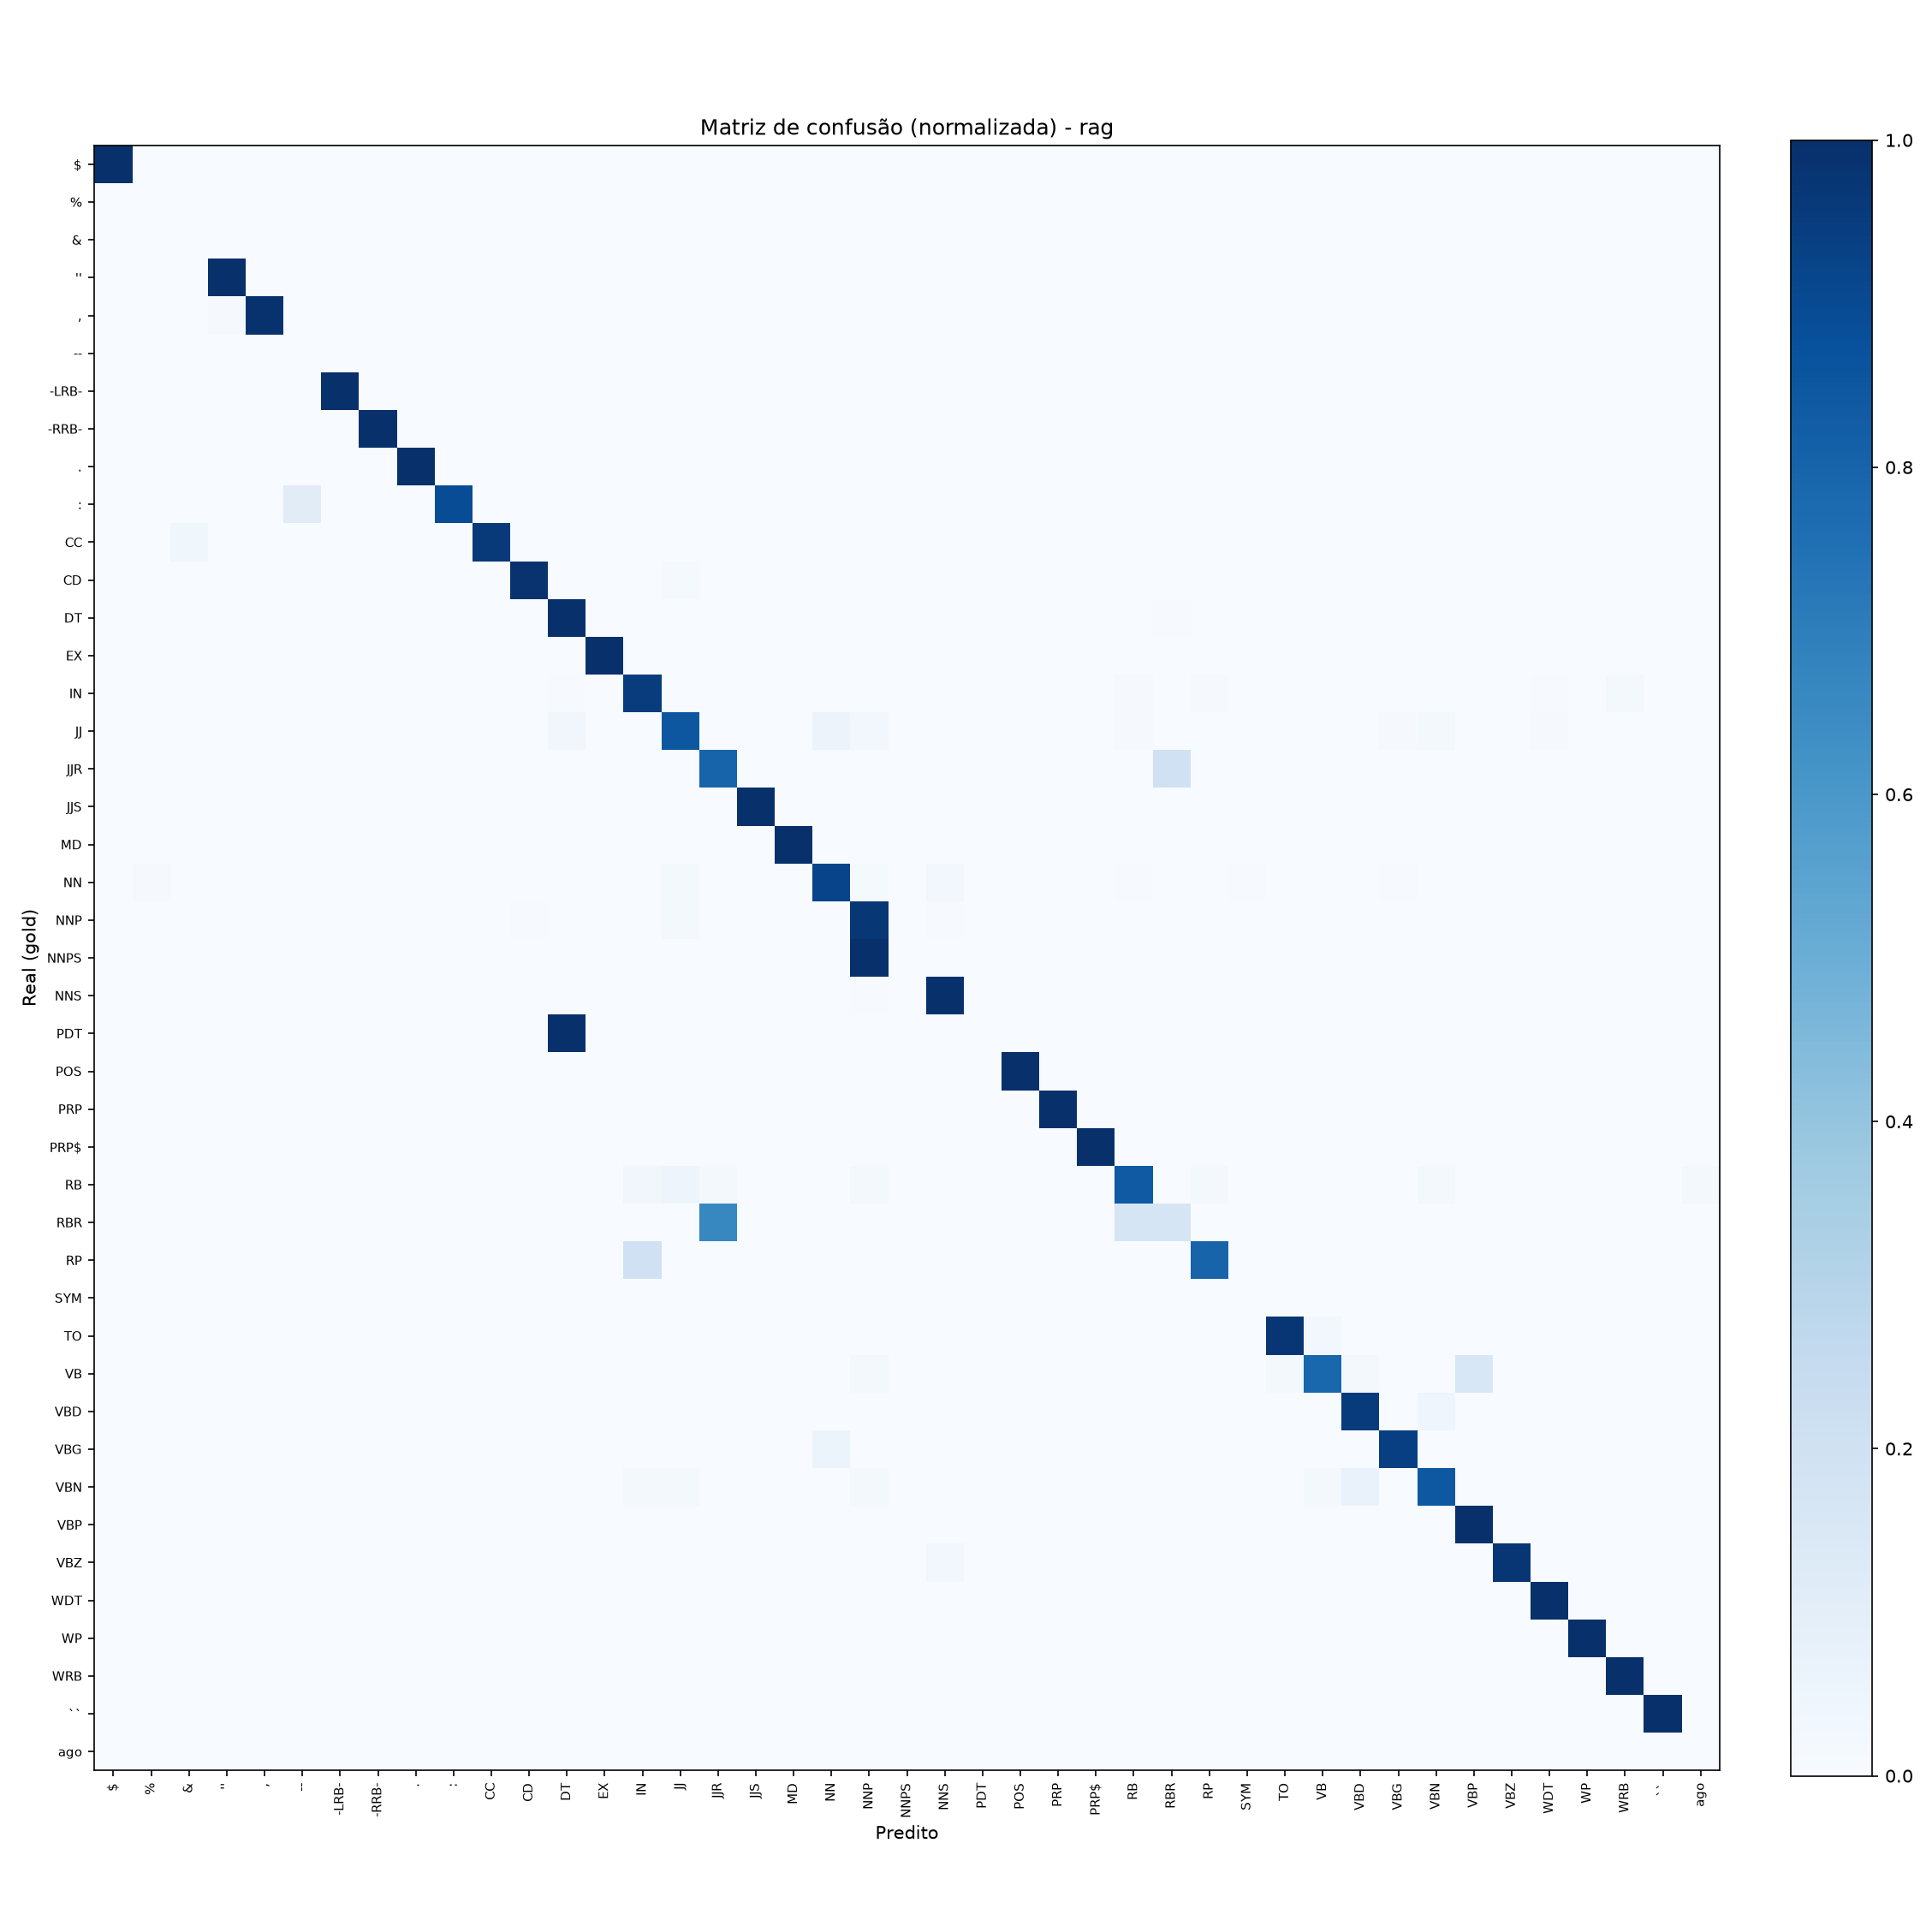
\includegraphics[width=0.9\textwidth]{images/confusion_matrix/rag.png}
    \caption{Matriz de Confusão da RAG.}
    \label{fig:rag}
\end{figure}

Um conjunto de confusões aparece de forma recorrente nos três modos, e corresponde a ambiguidades linguísticas conhecidas do tagset do PTB, não a erros aleatórios do modelo:

\begin{itemize}
    \item \textbf{$\text{JJR} \leftrightarrow \text{RBR}$ (adjetivo comparativo vs. advérbio comparativo):} "lower" pode assumir as duas funções dependendo do contexto sintático;
    \item \textbf{$\text{RB} \leftrightarrow \text{RP} \leftrightarrow \text{IN}$ (advérbio, partícula verbal e preposição):} a fronteira entre essas três categorias é um dos casos mais discutidos na literatura de anotação do PTB, por exemplo em verbos com partícula como "back" e "up";
    \item \textbf{$\text{VBD} \leftrightarrow \text{VBN}$ (passado simples vs. particípio):} formas homônimas como "recommended" exigem análise da estrutura da oração para retirar a ambiguidade;
    \item \textbf{$\text{NN} \leftrightarrow \text{NNP}$ e $\text{CD} \leftrightarrow \text{JJ/NN}$ ( substantivo comum vs. próprio, e numerais em função adjetival)}.
\end{itemize}

Esse padrão é consistente com a observação de Manning (2011) de que parte substancial do erro remanescente em tageadores de POS de alto desempenho decorre de ambiguidades linguísticas inerentes ao tagset, e não de limitações do classificador em si, o que sugere que os erros observados aqui não são exclusivos de LLMs, mas compartilhados por qualquer abordagem, estatística ou neural, treinada sobre o mesmo esquema de anotação. Além dessas confusões compartilhadas, cada modo também apresentou um padrão de erro específico:

\begin{itemize}
    \item No zero-shot, há uma confusão nítida entre WP e WDT (pronome interrogativo/relativo vs. determinante), quase ausente nos modos com exemplos, é uma evidência de que a demonstração de casos análogos ajuda o modelo a resolver essa ambiguidade fina. O zero-shot também confundiu o símbolo de dólar (\$) com um símbolo genérico (SYM) em um caso isolado;
    \item Ainda no zero-shot, o modelo produziu ao menos uma predição com a tag "PUNCT", que não existe no tagset do PTB (as tags corretas de pontuação são ".", ",", ":" etc., cada uma separada). Isso indica que, sem exemplos ancorando o formato exato solicitado, o modelo por vezes recorre a convenções de outros tagsets vistos durante o pré-treinamento em vez do tagset específico do PTB pedido no prompt;
    \item No RAG, houve ao menos um caso em que a predição retornada foi a própria palavra da sentença ("ago") em vez de uma tag. Um tipo de erro de formatação distinto do zero-shot: ao invés vez de inventar uma categoria, o modelo "vazou" o token de entrada para a saída;
\end{itemize}

Os exemplos few-shot e RAG parecem contribuir tanto para a acurácia de classificação quanto, de forma talvez mais decisiva, para a aderência ao formato e ao tagset exatos solicitados, o que está alinhado à conclusão de Min et al. (2022) de que os exemplos de demonstração comunicam o espaço de rótulos válidos e o formato geral esperado da saída, independentemente da correção específica de cada rótulo individual.

\subsubsection{Discussão dos Resultados}

O padrão geral observado ($\text{zero-shot} < \text{few-shot} \leq RAG$) está de acordo com a literatura de in-context learning, que consistentemente relata ganhos de desempenho ao se passar de zero-shot para few-shot (Brown et al., 2020). O que este trabalho acrescenta é uma decomposição desse ganho: a maior parte do salto de desempenho ocorre entre zero-shot e fewshot (+2,16 pontos percentuais), enquanto a diferença entre few-shot estático e RAG é pequena (+0,48 ponto percentual) e, como discutido anteriormente, não estatisticamente robusta nesta amostra.

Essa observação é compatível com o argumento de Min et al. (2022) de que boa parte do valor dos exemplos few-shot está em calibrar o modelo quanto ao espaço de rótulos e ao formato de saída esperado, e não necessariamente em fornecer contexto tematicamente relevante para cada instância, que é o diferencial teórico do RAG, segundo Liu et al. (2022) e Lewis et al. (2020). Neste experimento, ambas as fontes de exemplos (fixos ou recuperados) parecem ter cumprido bem essa função de calibração, o que ajuda a explicar por que a vantagem adicional do RAG sobre o few-shot estático foi discreta.

Uma hipótese complementar, específica deste corpus, é que o WSJ (Wall Street Journal) contém proporção considerável de sentenças com estrutura sintática padrão. Nesses casos, o RAG tende a recuperar exemplos quase idênticos em estrutura à sentença de teste, o que pode inflar artificialmente sua vantagem quando essas sentenças estão presentes na amostra avaliada, sem que isso generalize necessariamente para textos com menor redundância estrutural.


\section{Comparação entre Modelos}

Nesta seção, é feita uma síntese comparativa entre as arquiteturas, confrontando as expectativas iniciais com os resultados numéricos obtidos nos experimentos práticos.

A Tabela~\ref{tab:comparacao_modelos_final} organiza as características e as taxas de acurácia de cada modelo avaliado:

\begin{longtable}{p{4.5cm} p{2.2cm} C{2.5cm} p{6cm}}
\caption{Comparação final das arquiteturas e desempenho obtido.} \label{tab:comparacao_modelos_final} \\
\toprule
\textbf{Modelo/Arquitetura} & \textbf{Tarefa} & \textbf{Acurácia Real} & \textbf{Comportamento Sintético e Erros} \\ \midrule
\endhead
\bottomrule
\endfoot

\textbf{RNN Tradicional} & POS Tagging & 86,00\% & Apresenta limitações com dependências longas e viés para classes majoritárias. \\ \midrule
\textbf{LSTM Unidirecional} & POS Tagging & 87,00\% & Retenção de contexto histórico superior à RNN tradicional. \\ \midrule
\textbf{RNN Bidirecional} & POS Tagging & 86,00\% & Desempenho idêntico à versão unidirecional; não superou as limitações da célula. \\ \midrule
\textbf{LSTM Bidirecional} & POS Tagging & 90,00\% & Maior desempenho entre os modelos recorrentes devido ao fluxo bidirecional. \\ \midrule
\textbf{Transformer Decoder-Only} & POS Tagging & 92,77\% & Desempenho inferior aos outros Transformers devido ao uso de máscara causal. \\ \midrule
\textbf{Transformer Encoder-Only} & POS Tagging & 93,93\% & Boa capacidade de classificação local através de atenção bidirecional plena. \\ \midrule
\textbf{Transformer Encoder-Decoder} & POS Tagging & \textbf{94,40\%} & \textbf{Maior acurácia do projeto}. Separação eficiente entre os embeddings de palavras e tags. \\ \midrule
\textbf{LLM Comercial (Zero-shot)} & POS Tagging & 91,75\%* & Boa base gramatical, mas registrou 15\% de falhas no formato JSON solicitado. \\ \midrule
\textbf{LLM Comercial (Few-shot)} & POS Tagging & 93,91\%* & Exemplos estáticos reduziram falhas de formato e ajudaram em tags ambíguas (\texttt{WP} vs. \texttt{WDT}). \\ \midrule
\textbf{LLM Comercial (RAG)} & POS Tagging & 94,39\%* & Desempenho próximo ao few-shot fixo, com sobreposição dos intervalos de confiança. \\
\bottomrule
\end{longtable}
\small{*Nota: Os índices das LLMs desconsideram as sentenças que falharam na geração do formato JSON exigido.}

\subsection{Análise dos Resultados em Relação às Hipóteses}

O confronto entre as expectativas teóricas e os dados empíricos aponta as seguintes observações:

\begin{enumerate}
    \item \textbf{Desempenho das Variações de Transformer:} Inicialmente, estimava-se que o modelo \textit{Encoder-Only} seria o mais adequado para a marcação de tags. Contudo, o \textit{Encoder-Decoder} obteve uma acurácia ligeiramente superior (94,40\% contra 93,93\%). Os testes sugerem que isolar a geração das etiquetas no Decoder, utilizando embeddings menores (64d), gerou um efeito de regularização útil para a tarefa.
    \item \textbf{Efeito do Contexto Unidirecional:} Confirmando o esperado, modelos que operam com restrição de contexto futuro (como as redes recorrentes unidirecionais e o \textit{Transformer Decoder-Only}) obtiveram desempenhos inferiores às suas contrapartes bidirecionais. A classificação morfológica de termos em inglês mostra-se dependente da leitura das palavras subsequentes na oração.
    \item \textbf{Comparação entre LLM e Modelos Treinados:} O método de aprendizado em contexto utilizando a LLM Comercial com \textit{RAG} obteve uma acurácia de 94,39\% (considerando apenas saídas válidas), o que se equipara ao desempenho do melhor Transformer treinado do zero (94,40\%). Essa abordagem mostrou-se competitiva em acurácia linguística, embora demande mecanismos externos para tratar as taxas de erro na formatação da saída (que variaram entre 11\% e 15\% nos testes).
\end{enumerate}
\newpage
\addcontentsline{toc}{section}{Bibliografia}
\begin{thebibliography}{9}

\bibitem{jurafsky_nlp}
Daniel Jurafsky and James H. Martin; Speech and Language Processing: An Introduction to Natural Language Processing, Computational Linguistics, and Speech Recognition, with Language Models. 2026. 3rd Edition

\bibitem{dsa_deeplearning}
Equipe DSA. Deep Learning Book. Disponível em: https://www.deeplearningbook.com.br/. Acesso em: 22 out. 2025.

\bibitem{razvan_rnn}
PASCANU, Razvan.; MIKOLOV, Tomas; BENGIO, Yoshua.  On the difficulty of training Recurrent Neural Networks. arXiv preprint arXiv: 1211.5063, 2012. Disponível em: https://arxiv.org/abs/1211.5063. Acesso em: 21 jun. 2026.

\bibitem{aston_deeplearning}
ZHANG, Aston; LIPTON, Zachary C.; LI, Mu; SMOLA, Alexander J. Dive into Deep Learning. 2021. Disponível em: https://pt.d2l.ai/chapter\_preface/index.html. Acesso em: 21 jun. 2026.

\bibitem{mike_bidirectional_rnn}
Schuster, Mike and Paliwal, Kuldip. (1997). Bidirectional recurrent neural networks. Signal Processing, IEEE Transactions on. 45. 2673 - 2681. 10.1109/78.650093.


\end{thebibliography}

\end{document}
